\section{Object Reconstruction}\label{sec:reconstruction}
The outputs from the CMS detector, after some processing of the raw signals, are essentially, hits in the tracking systems and energy deposits in the calorimeters. To perform a physics analysis, we want to identify what physics objects were produced in the collisions and what their properties were. Physics objects include electrons, muons, taus, photons and jets. An example of an important property is the four-momentum of the object. The process of interpreting the outputs of the detector as physics objects is known as \textit{reconstruction}. 

In the CMS experiment, object reconstruction begins with the particle-flow (PF) algorithm and its creation of the basic \textit{elements}: tracks and energy clusters~\cite{CMS:2017yfk}. These elements are \textit{linked} within and across detector systems to form \textit{blocks} of elements, which are then used to create object candidates. By combining information across systems, the particle-flow algorithm is able to create object candidates with great resolution and efficiency and this concept was key to the design of the algorithm. Further details on tracking, clustering and the link algorithm are provided in \cref{sec:tracking,sec:calo_clustering,sec:link_algorithm}.

PF object candidates are input to specialized algorithms that complete the object reconstruction. In most cases, these algorithms are used to apply final identification criteria and calibration but in some cases, they also create more complex objects such as jets. These algorithms are described in \cref{sec:muon_reco,sec:eg_reco,sec:jet_reco,sec:tau_reco} where details are restricted to those which are most relevant to the di-Higgs search in \cref{chap:dihiggs}. 

\subsection{Tracking}\label{sec:tracking}
The algorithm~\cite{Adam:2005cg,Cucciarelli:2006mt,CMS:2014pgm,Elmetenawee:2023xyl} for reconstructing tracks in the inner tracker is based on the combinatorial Kalman filter (CKF)~\cite{Fruhwirth:1987fm,Billoir:1989mh,Billoir:1990we,Mankel:1997dy}. Initially, tracking seeds are generated from a few hits consistent with a charged-particle trajectory. The seeds provide a coarse estimate of the track trajectory and from that, the CKF propagates through the tracker, looking for compatible hits in each tracker layer and updating the trajectory estimate as it does so. If multiple compatible hits are found in a layer, the CKF will create multiple track candidates and propagate them all (hence combinatorial). After exhausting all tracker layers, the tracks are refitted with greater precision and then selected based on quality criteria such as the number of hits and the $\chi^2$ of the fit. 

Given the combinatorial nature of the algorithm, CKF can be computationally expensive. This could be handled by, for example, only propagating tracks that have a high \pt or that coincide with the interaction point, but this would lead to a loss of efficiency for low \pt tracks or tracks that originate from displaced vertices. To mitigate this, an iterative approach is used where multiple runs of the CKF are performed, with varying types of seeds and selection criteria which target different types of tracks, for example, high \pt in one run and displaced tracks in the next. After each stage, the hits associated with the selected tracks are removed from the list of hits available to the CKF. This reduces the combinatorial complexity of the problem and allows the CKF to focus on the remaining hits. Ultimately, this iterative approach leads to higher reconstruction efficiency whilst keeping the misconstruction rate low~\cite{CMS:2017yfk}.

In the muon systems, a separate Kalman-filter based algorithm is used to reconstruct \textit{standalone-muon} tracks~\cite{CMS:2018rym}. These muon tracks can then be matched with inner tracks to create \textit{global-muon} tracks. Similarly, inner tracks are propagated to the muon system to create \textit{tracker-muon} tracks. Due to the high reconstruction efficiency in the inner tracker and muon systems, about 99\% of muons within the geometrical acceptance of the muon systems are reconstructed as global muons or tracker muons, and often as both~\cite{CMS:2017yfk}.

Electrons emit a sizeable fraction of their energy as bremsstrahlung photons before reaching the ECAL. If the momentum of an electron changes enough along its trajectory, the iterative CKF algorithm can fail to reconstruct the track. Therefore, for electrons, a Gaussian Sum Filter (GSF) algorithm is instead used which allows for more sudden and significant energy losses along the particle's path~\cite{Adam:2003kg}.
\subsection{Calorimeter Clustering}\label{sec:calo_clustering}
Energy deposits in the calorimeters are grouped into \textit{clusters} where each cluster is hypothesized to originate from a single particle incident on the ECAL~\cite{CMS:2017yfk}. The clustering is performed independently in the ECAL barrel, ECAL endcaps, HCAL barrel, HCAL endcaps, Preshower and the HF. In the HF, the electromagnetic and hadronic components of each cell directly give rise to separate clusters. In the rest of the calorimeters, a more complex algorithm is used which is described below.

First, cluster seeds are identified as cells with energy larger than a given threshold and larger than any neighbouring cells, where neighbouring cells are the four cells that share a side with the seed cell or the eight cells that share a side or corner, depending on the calorimeter system. The seed cells are then grown into \textit{topological clusters} by adding cells that share a corner and have an energy of at least twice the noise level of the cell. 

Particles that are close to each other in $\eta$-$\phi$ space can have overlapping energy deposits, which in turn, can lead to a topological cluster having multiple seeds. In these cases, the energies from the cells are split and shared amongst the seeds. This is done using a Gaussian-mixture model that postulates that the energy deposits in the $M$ individual cells come from $N$ different Gaussian energy deposits, one for each seed. After fitting the model, the energy and positions of the $N$ Gaussian deposits are taken as cluster parameters~\cite{CMS:2017yfk}.

Electrons and photons have a significant probability of undergoing bremsstrahlung radiation or photon conversion prior to reaching the ECAL leading to several distinct clusters in the ECAL. To measure the energy of the original electron or photon, the clusters are grouped into a \textit{supercluster} which is then used to create the electron or photon candidate. A supercluster (SC) is first formed by including all clusters in an \ET-dependent zone in $\phi-\eta$ space centred around the seed cluster~\cite{CMS:2020uim}. Then, a conversion-finding algorithm~\cite{CMS:2008xjf} is used to identify tracks and associated ECAL deposits consistent with a photon conversion. Furthermore, at each tracker layer, tangents from an electron's trajectory are extrapolated to look for clusters from bremsstrahlung photons. All of this information is then fed into the PF link algorithm which builds electron and photon candidates.
\subsection{Link Algorithm}\label{sec:link_algorithm}
After the creation of the PF elements (tracks and clusters), a linking algorithm is used to form particle candidates by creating associations between elements that are likely to have originated from the same particle~\cite{CMS:2017yfk}. Firstly, inner tracks are linked to calorimeter clusters when the track's extrapolated trajectory overlaps with the cluster. Similarly, clusters in different calorimeters are linked if the cluster's centre from the calorimeter with greater granularity is within the cluster of the calorimeter with coarser granularity. If there are multiple possible links, the link with the smallest distance in $\phi$-$\eta$ space, or $x$-$y$ space for ECAL-Preshower links, is chosen. Finally, links between tracks can be created if the tracks share a common secondary vertex.

Particle candidates are now formed sequentially, starting with muons, then electrons and photons, then charged and neutral hadrons~\cite{CMS:2017yfk}. Identification of muons and photons are also revisited at later stages to recover candidates that were missed by initially stringent criteria. At each stage, the PF elements related to the particle candidates are removed from the list of elements available to the link algorithm. This ensures that the algorithm does not link the same element to multiple candidates and that the same element is not used to create multiple candidates. Finally, an event post-processing step is performed to correct for artificially-large \ptmiss~\cite{CMS:2017yfk}.
\subsection{Muons}\label{sec:muon_reco} 

\subsubsection{Muon Identification}

In CMS, there are five main identification (ID) types for muons: loose, medium, tight, soft, and high momentum~\cite{CMS:2018rym}. Each type is defined by cuts on a number of variables including the track fit $\chi^2$, number of hits per track, the compatibility of the muon track with the PV, the compatibility of the inner track with the standalone muon track (for global muons), and a related quantity called muon segment compatibility~\cite{CMS:2009fdy} which takes a value between 0 and 1 where 1 represents high compatibility. Additionally, a kink-finding algorithm is used to discriminate against charged hadrons which are more likely to interact with the tracker material than muons are. This algorithm, at several places along the track, splits the inner track (if present) in two and tests if the two halves are compatible with a single track.

The loose muon ID is designed to have a low efficiency for hadrons, and to select muons originating from the interaction vertex (prompt muons) or from light and heavy flavour decays. It is defined as a muon selected by the PF algorithm which is a tracker or global muon. The medium muon ID, which is used in the di-Higgs search in \cref{chap:dihiggs}, is designed for prompt muons and muons from heavy flavour decay. A medium muon is a loose muon which passes the following additional requirements: 
\begin{itemize}
  \setlength{\itemsep}{-3pt}
  \item has an inner track with hits from more than 80\% of the tracker layers it traverses;
  \item if the muon is only a tracker muon, the muon segment compatibility must be greater than 0.451;
  \item if the muon is a global muon, the muon segment compatibility must be greater than 0.303 and the global track fit $\chi^2/\text{dof}$ must be less than 3;
  \item the position match between the inner track and the standalone muon track must have $\chi^2 < 12$;
  \item and the maximum $\chi^2$ computed by the kink-finding algorithm must be less than 20.
\end{itemize}
These requirements were tuned to provide an identification efficiency of 99.5\% for muons in simulated $\PW\to\mu\nu$ and $\PZ\to\mu\mu$ events~\cite{CMS:2018rym}. 

The tight muon ID is designed to suppress muons from decay in flight and from hadronic punch-through, the soft muon ID is designed for low-\pt muons from b-hadron decays, and the high momentum muon ID is designed for muons with \pt greater than 200\GeV. The definition for these IDs can be found in Ref.~\cite{CMS:2018rym}. 

Further requirements can also be made on the particle-flow isolation, \IPF, of the muon, which is defined as the pileup-corrected sum of the \pt of the charged hadrons, photons, and neutral hadrons in a cone of $\dR < 0.3$ around the muon. The pileup correction subtracts the expected contribution originating from pileup interactions. Tight and loose working points are defined to achieve muon ID efficiencies of 95\% and 98\% respectively in simulated $\PZ\to\mu\mu$ events~\cite{CMS:2018rym}.

Reconstruction, identification, and isolation efficiencies are measured in data and compared to simulation. The ratio of the efficiencies, referred to as \textit{scale factors}, are then used to correct the simulation to match data by multiplying the simulation events weights by these factors. These scale factors are derived separately for each year of data-taking to account for varying detector conditions, and in bins of muon \pt and $\eta$ to account for the dependence of the muon kinematics and detector geometry on the simulation mismodelling. The full details of the derivation of these scale factors can be found in Refs.~\cite{CMS:2018rym,CMS:2019ied,CMS-DP-2017-007,CMS-DP-2018-042,CMS-DP-2019-022,CMS-DP-2020-040}. 

As an example, the efficiency of the medium muon ID as measured in data and simulation for 2018 is shown in \cref{fig:muon_id_performance} for two $\eta$ regions. For $\abs{\eta} < 0.9$, the efficiency in simulation is about 99.5\% as expected, and in data is slightly lower, at about 99\%. For $2.1 < \abs{\eta} < 2.4$, where fewer inner tracker hits are expected due to the tracker geometry (see \cref{fig:tracker}) the efficiency is lower at about 99\% and 96\% for simulation and data respectively. In both cases, and especially for $2.1 < \abs{\eta} < 2.4$, there is disagreement between data and simulation, highlighting the need for scale factors.

\begin{figure}
    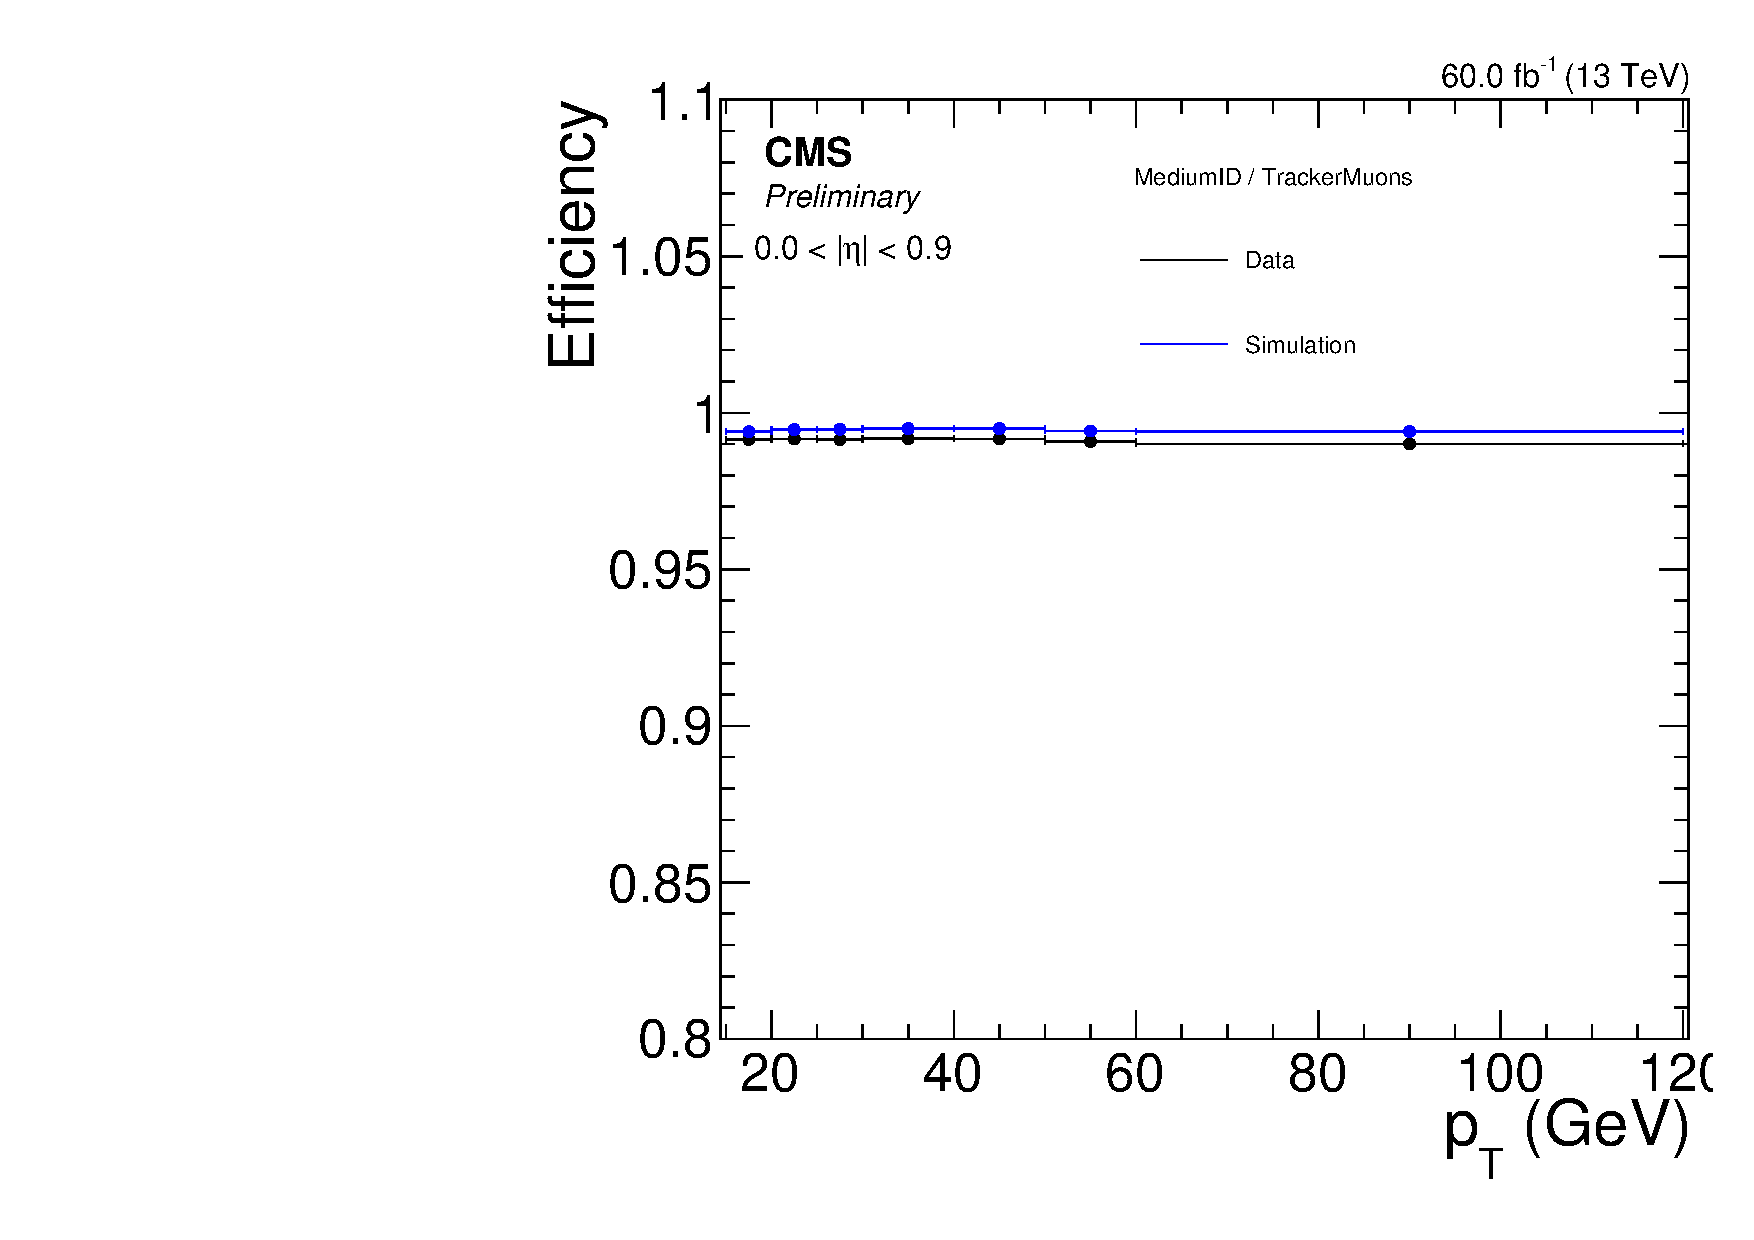
\includegraphics[width=0.49\textwidth]{Figures/Detector/CMS/muon_id_low_eta.pdf}
    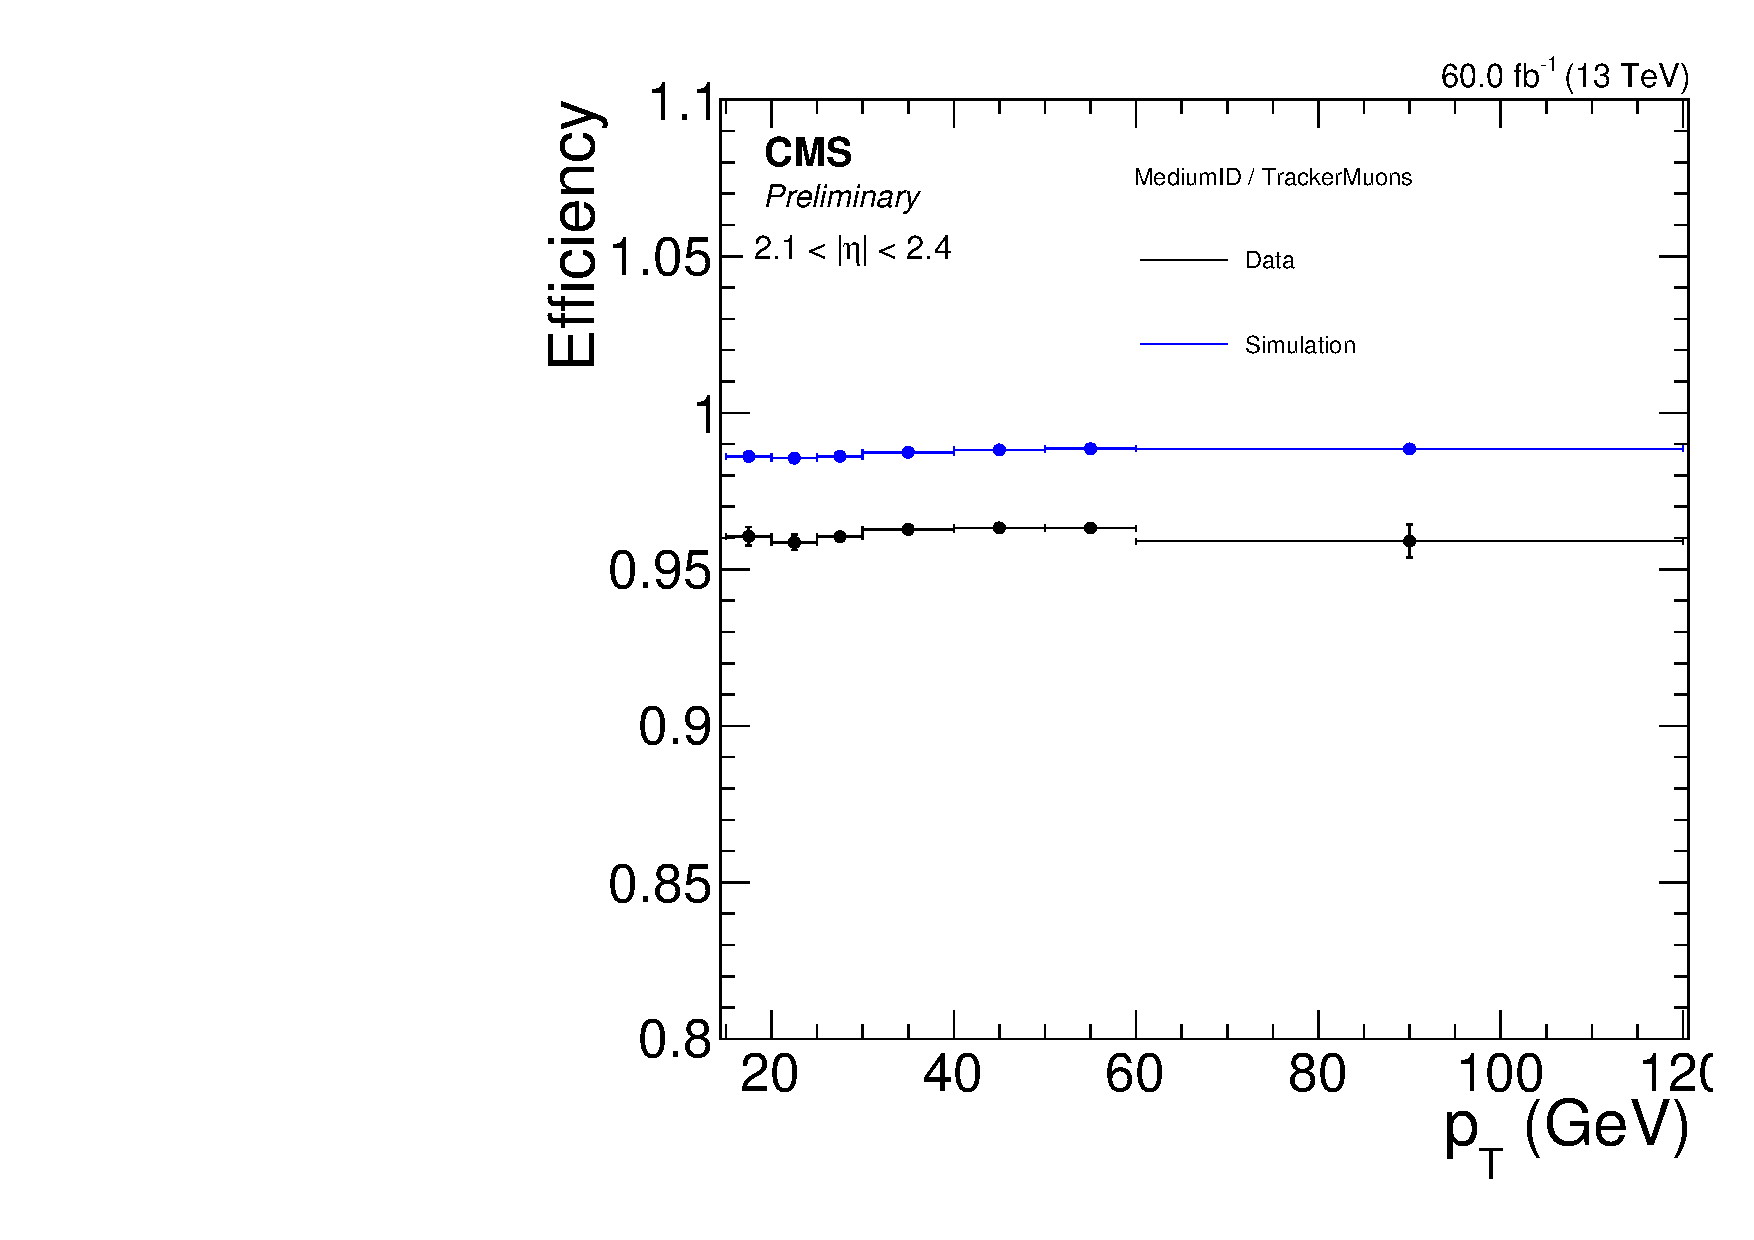
\includegraphics[width=0.49\textwidth]{Figures/Detector/CMS/muon_id_high_eta.pdf}
    \caption[Medium Muon ID Efficiency in 2018]{Medium muon ID efficiency in 2018 as measured in data and simulation as a function of muon \pt for $\abs{\eta} < 0.9$ (left) and $2.1 < \abs{\eta} < 2.4$ (right).}\label{fig:muon_id_performance}
  \end{figure}

\subsubsection{Muon Momentum}

Muon momentum is determined by the Tune-P algorithm~\cite{CMS:2012nsv} which selects the \pt measurement from different refits of the muon track based on the goodness-of-fit information and estimated \pt resolution. The types of refits include tracker-only, tracker and first muon detector plane, global without muon chambers with high occupancies, and a \textit{dynamic-truncation} fit which propagates the track to the muon stations but stops as soon as no compatible hit is found in two consecutive stations.

The momentum scale calibration and resolution estimation are derived from $\PZ/\gamma^*\to\mu\mu$, $J/\psi\to\mu\mu$ and $\Upsilon(1S)\to\mu\mu$ events in data~\cite{Bodek:2012id}. The momentum scale corrections are about 0.2\% and 0.3\% in the barrel and endcap respectively, and the resolution is about 1\% in the barrel and 3\% in the endcap for muons with \pt up to 100\GeV. The momentum resolution of intermediate and high \pt muons is additionally measured in cosmic ray events by comparing the momentum measurements in the upper and lower halves of the detector~\cite{CMS:2009fdy}. The momentum resolution, as measured with this method in 2015 data, is shown in \cref{fig:muon_resolution}. 

\begin{figure}
  \centering
  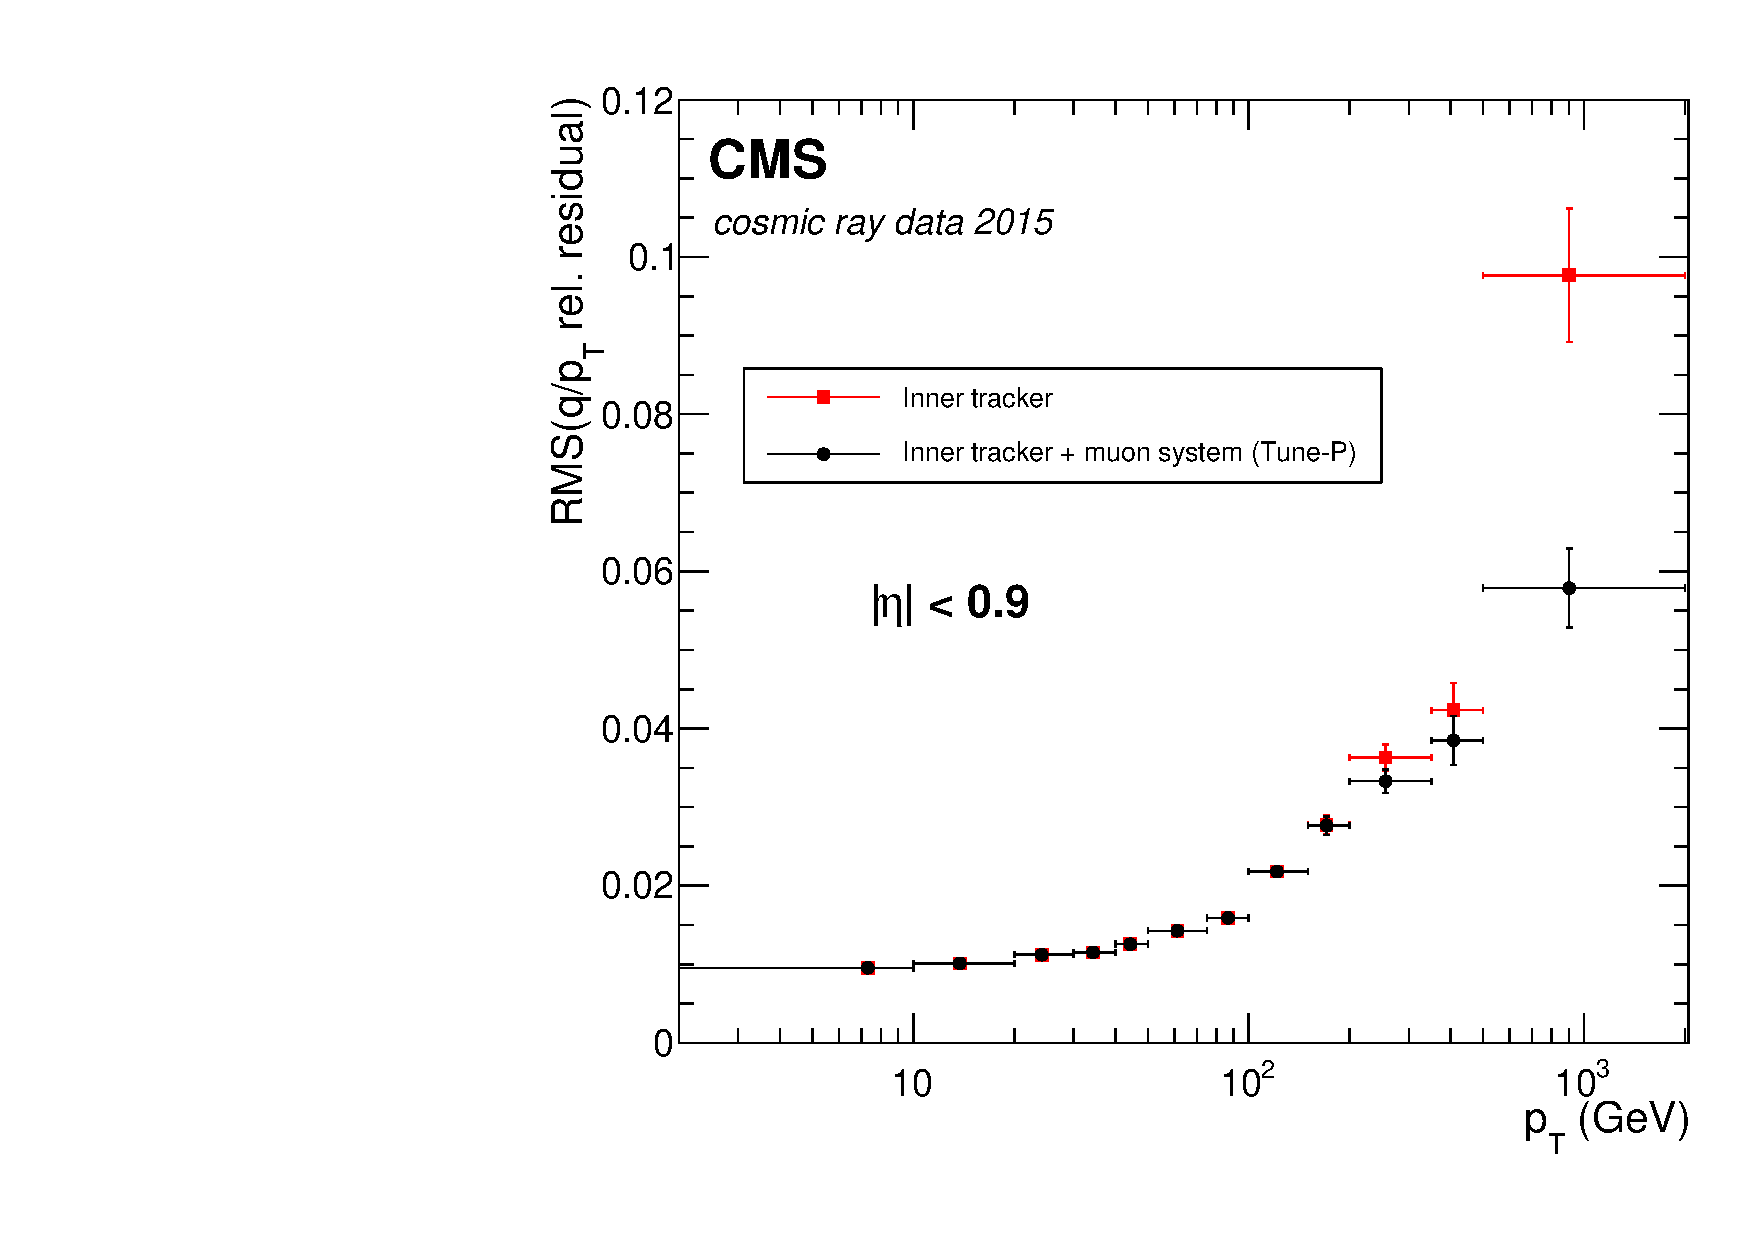
\includegraphics[width=0.7\textwidth]{Figures/Detector/CMS/muon_momentum_resolution.pdf}
  \caption[Muon Momentum Resolution as a Function of \pt]{Relative muon momentum resolution as a function of \pt for $\abs{\eta} < 0.9$ measured using cosmic ray data collected in 2015. The vertical error bars indicate statistical uncertainties. Figure taken from Ref.~\cite{CMS:2018rym}.}\label{fig:muon_resolution}
\end{figure}
\subsection{Electrons and Photons}\label{sec:eg_reco}
Electrons and photons share many of the same reconstruction and identification algorithms because, with the exception of an electron's track, the two particle leave similar signatures in the detector. Both particles are expected to be contained within the ECAL, and have almost identical showering properties. In this section, reconstruction for electron and photon ($\eg$) objects will be described together, with differences highlighted where necessary.

\subsubsection{Electron and Photon Identification}\label{sec:eg_id}

Background sources for prompt electrons include photon conversions, hadrons misidentified as electrons, and secondary electrons from semileptonic decays of b or c quarks. Background sources for prompt photons are primarily secondary photons from light neutral mesons ($\pi^0$ and $\eta$). Using variables related to the isolation and shower shape of the electrons and photons, multivariate (MVA) discriminators are trained to separate real electrons and photons from these background sources~\cite{CMS:2020uim}. Additional tracker-related variables are also used for the identification of electrons.

The isolation variables are constructed by considering a cone of $\dR<0.3$ around the \eg candidate and summing the \pt of the charged hadrons (\Ich), photons (\Iph), and neutral hadrons (\In) inside the cone. As is done for \IPF, a pileup correction is applied in these sums, and these variables are useful for discriminating against backgrounds originating from jets. Another important variable is the ratio of energy of associated HCAL clusters to the supercluster energy (H/E), which is expected to be lower for \eg objects than for hadrons.

The shower shape variables exploit differences in the showering of prompt \eg objects from photons from neutral hadron decays, which are expected to have a wider profile on average. One such variable is $\sigma_{i\eta i\eta}$, which is the standard deviation of the shower in $\eta$ in terms of the absolute number of crystal cells~\cite{CMS:2020uim}. Another important variable is \RNINE, which is a measure of how localized the energy deposit is, and is defined as the ratio of the energy of the $3\times3$ cell grid surrounding the SC seed to the energy of the SC. For electrons, variables related to the compatibility of the track with the SC are also used which include the differences between the energy, $\eta$ and $\phi$ of the electron, measured by the track and the SC.

These discriminating variables are combined into single discriminators using BDTs. This is done separately for electron and photons and the BDTs are trained on simulated DY + jets and $\gamma$ + jets events for electrons and photons respectively. In both cases, the dependence on $\eta$ and \ET is included, either by introducing these variables as inputs to the BDT, or by training several BDTs in different bins of $\eta$ and \ET. The performance of these algorithms as measured by simulation for 2017 is shown in \cref{fig:eg_id_performance}. Two working points are defined: WP90 and WP80, corresponding to signal efficiencies of about 90\% and 80\% respectively and physics analyses are left to choose which point to use based upon their level of background. 

\begin{figure}
  \includegraphics[width=0.49\textwidth]{Figures/Detector/CMS/electron_id_performance.pdf}
  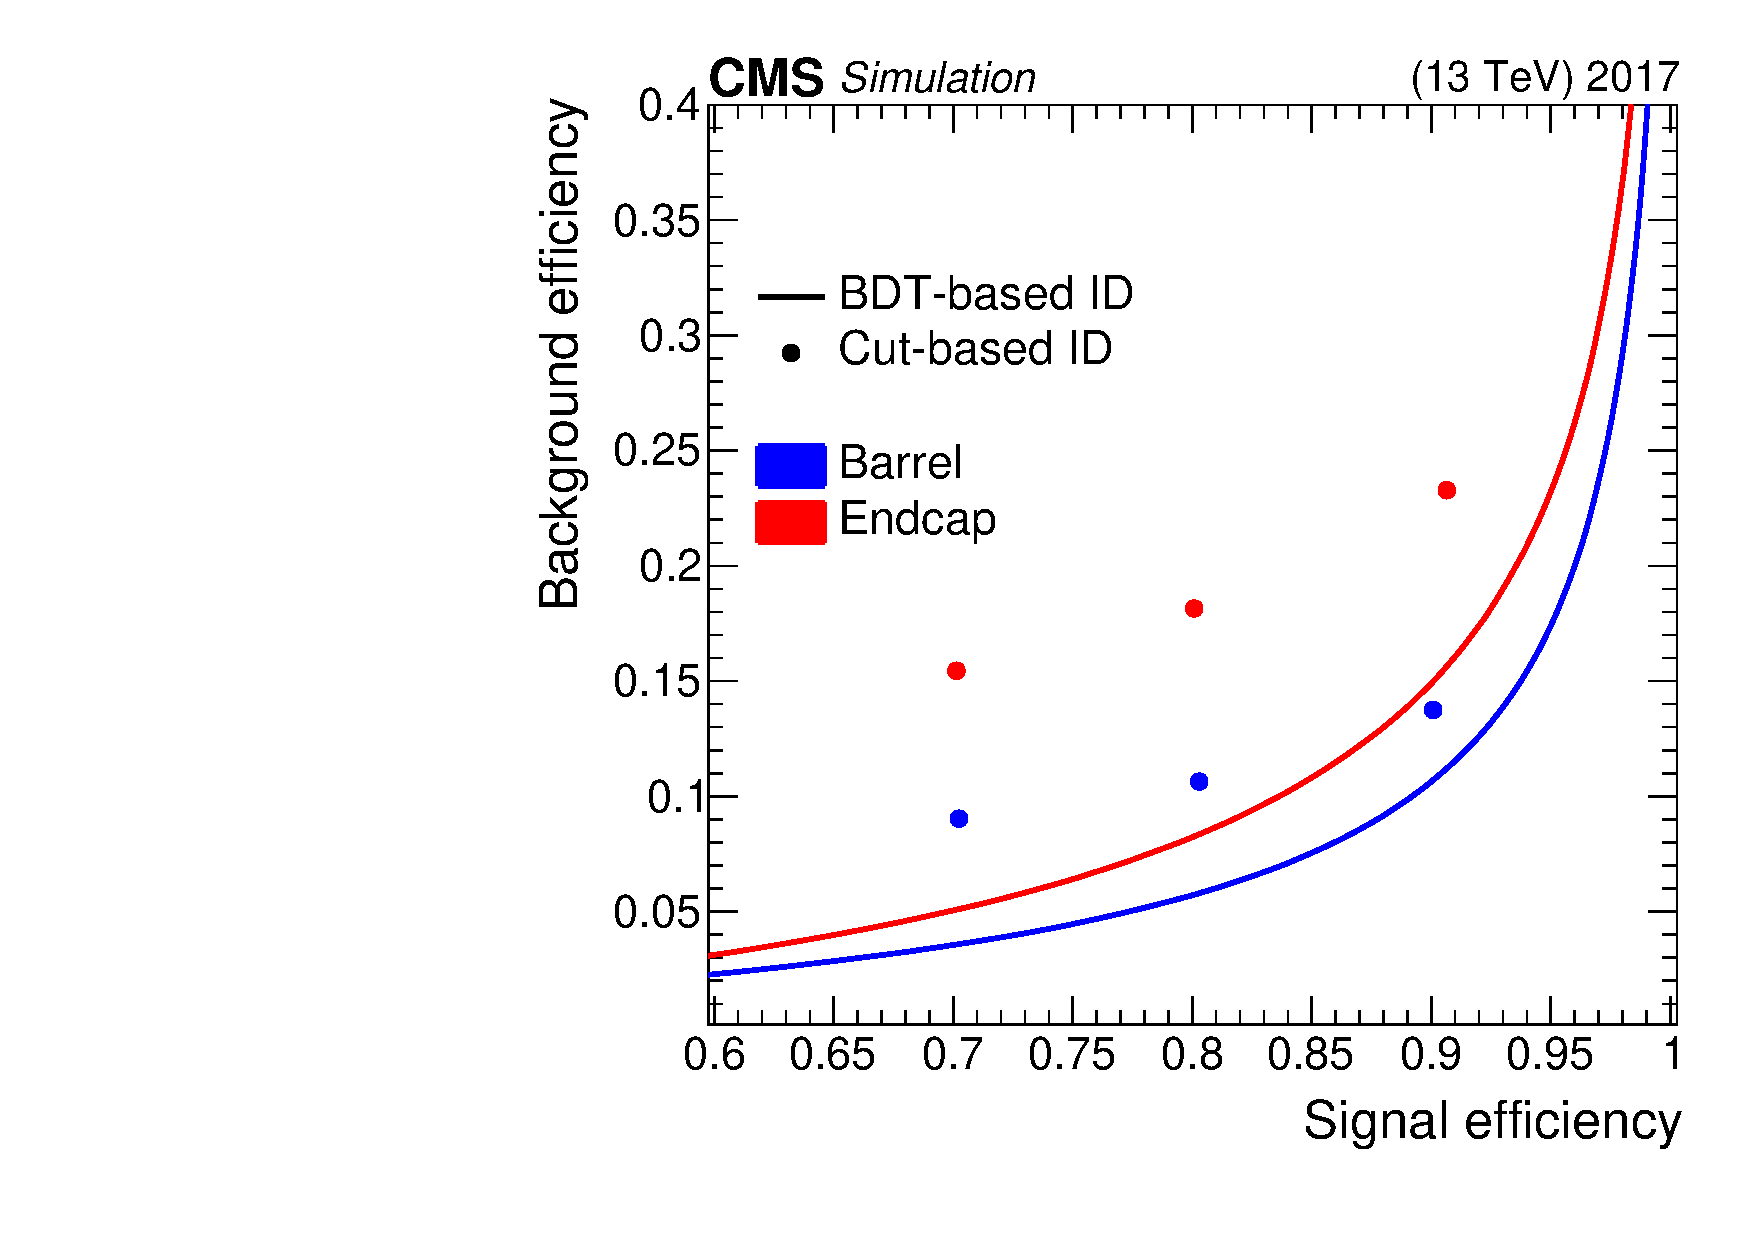
\includegraphics[width=0.49\textwidth]{Figures/Detector/CMS/photon_id_performance.pdf}
  \caption[Electron and Photon Identification Performance]{Performance of the electron (left) and photon (right) IDs in the ECAL barrel and endcaps evaluated for 2017 with simulated events. Different algorithms are shown for comparison's sake. For electrons, three algorithms are shown: a BDT trained without the isolation variables, the same BDT with isolation cuts applied separately, and a BDT with isolation variables included in training, where the last algorithm is the most performant. For photons, BDT-based and cut-based IDs are shown where the former is the most performant. Figures taken from Ref.~\cite{CMS:2020uim}.}\label{fig:eg_id_performance}
\end{figure}

The electron ID efficiencies are measured in data using $\PZ\rightarrow ee$ events. The photon ID efficiencies are also measured in $\PZ\rightarrow ee$ events, where the electrons are reconstructed in the same way as photons by omitting the information from the electron track. This is motivated by the fact that electrons and photons shower similarly in the ECAL and is validated using $\PZ\rightarrow\mu\mu\gamma$ events. The measured electron and photon ID efficiencies and a comparison to simulated efficiencies are shown for the WP90 working points in \cref{fig:eg_id_data_mc}. Scale factors are derived separately for each year and in bins of $\eta$ and \ET to correct the simulation to match data, and are up to 5\%~\cite{CMS:2020uim}. 

\begin{figure}
  \centering
  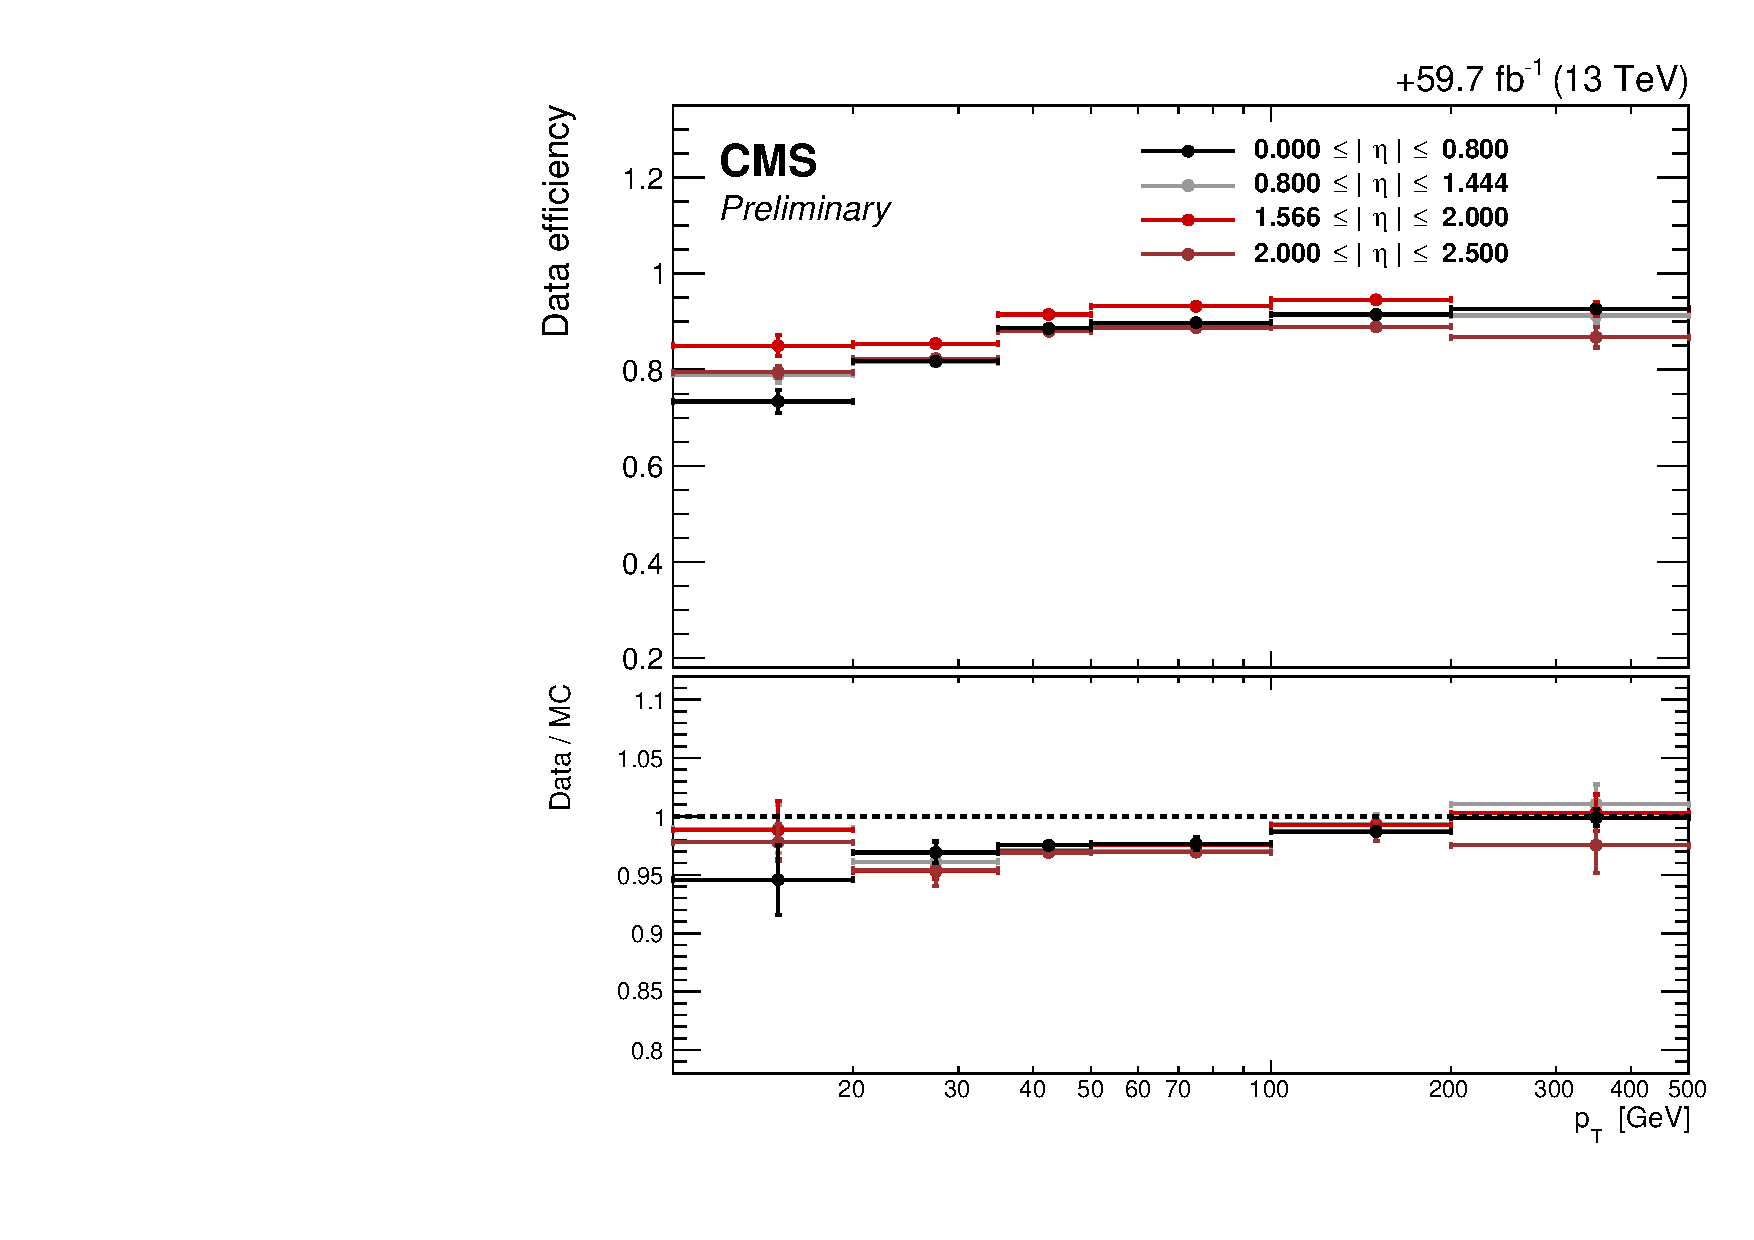
\includegraphics[width=0.60\textwidth]{Figures/Detector/CMS/electron_id_data_mc.pdf} \\
  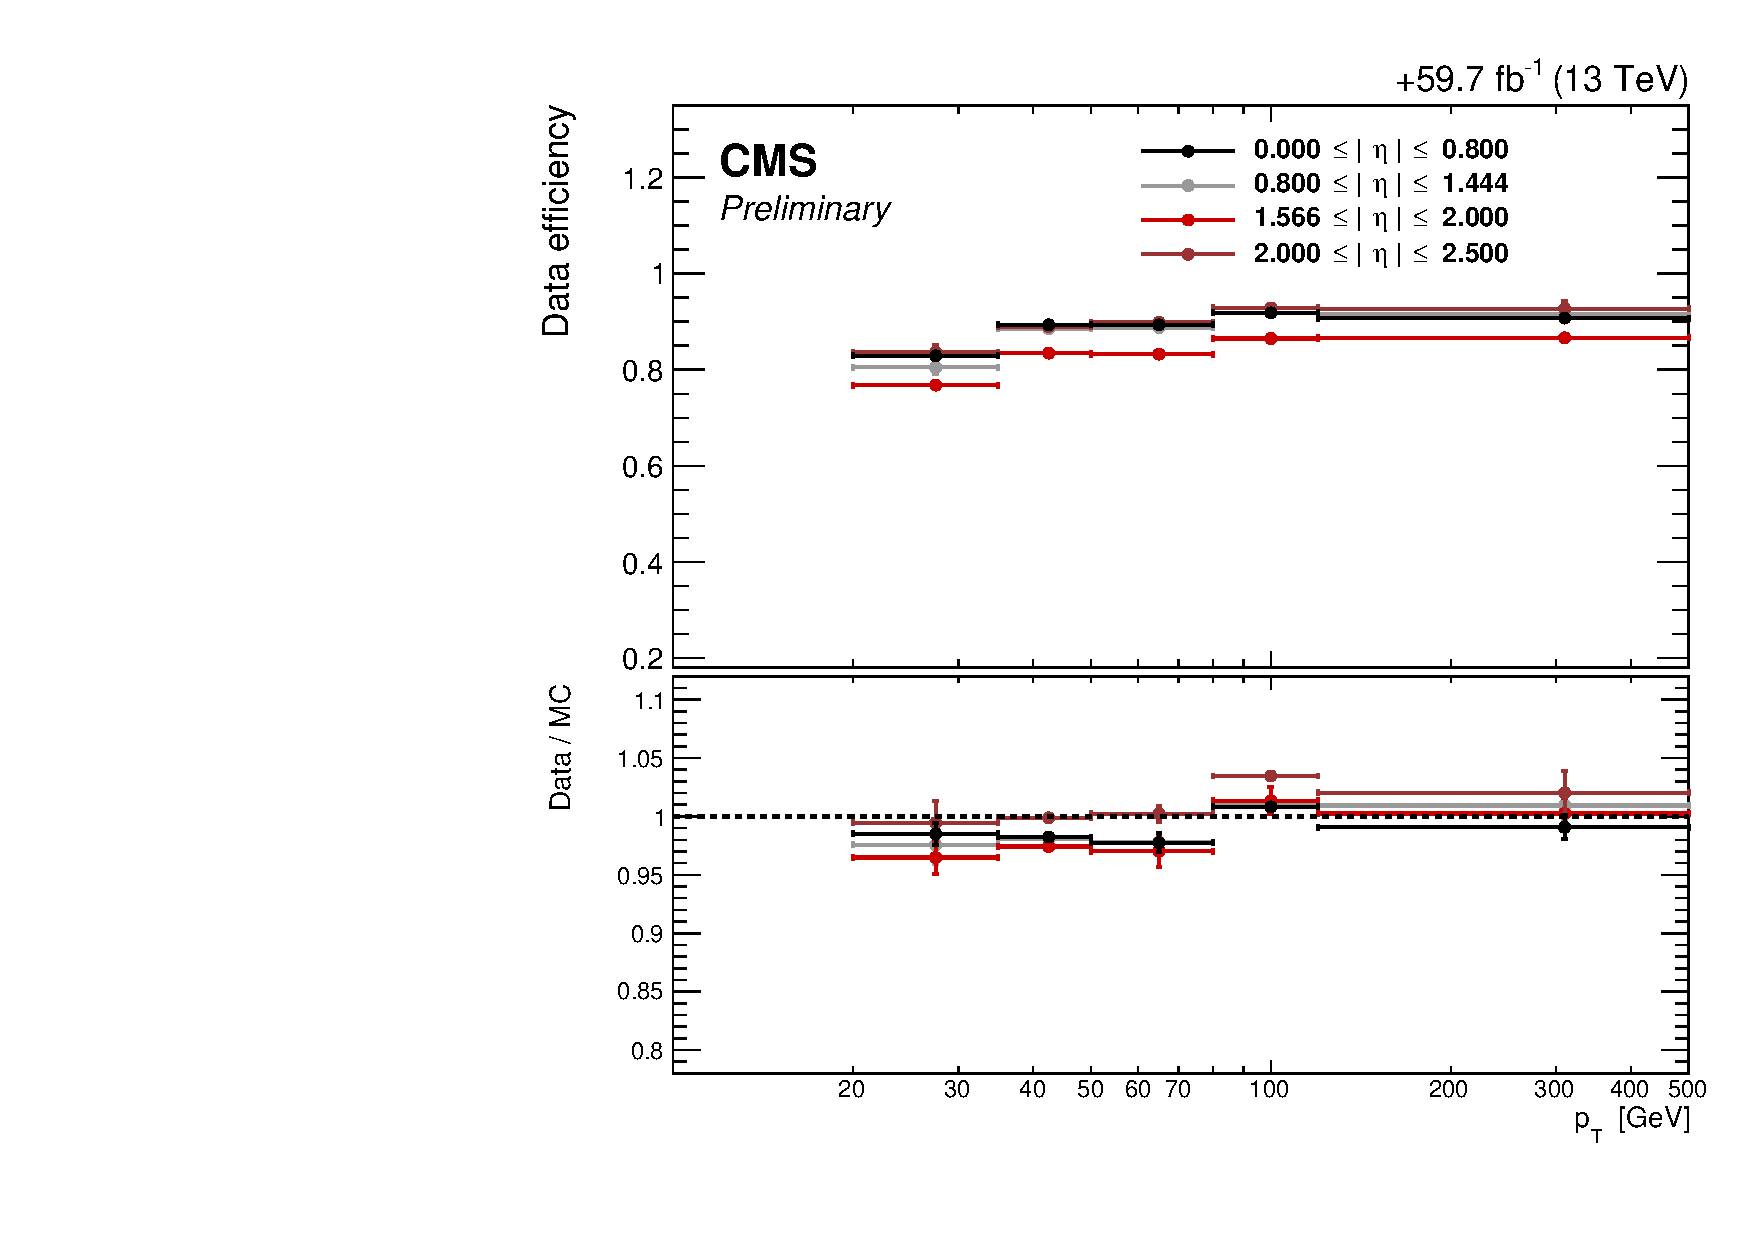
\includegraphics[width=0.60\textwidth]{Figures/Detector/CMS/photon_id_data_mc.pdf}
  \caption[Signal Efficiencies of Electron and Photon Identification Algorithms for the WP90 Working Point, Measured in Data and Simulation]{Signal efficiencies of the electron (top) and photon (bottom) BDT IDs at the WP90 working points. In the top halves of each figure, the efficiencies as measured in 2018 data with $\PZ\to ee$ events are shown. In the bottom halves, the ratio of the efficiencies in data to simulation (scale factors) are shown. The vertical error bars indicate combined statistical and systematic uncertainties. Figures taken from Ref.~\cite{CMS:2020uim}.}\label{fig:eg_id_data_mc}
\end{figure}

Finally, when searching for photon candidates, a conversion-safe electron veto (CSEV) can be used~\cite{CMS:2015myp}. This veto requires that there are no charged-particles tracks pointing to the photon SC, where the tracks are required to have a hit in the first layer of the pixel detector, and are not matched to a reconstructed conversion vertex. This leads to photon and electron efficiencies of about 99\% and 5\% for the barrel, and 98\% and 20\% for the endcap respectively. An even more stringent veto, the \textit{pixel veto}, rejects any photon where there exists at least two pixel hits that form a track pointing to the SC. This leads to photon and electron efficiencies of about 95\% and 1\% for the barrel, and 80\% and 5\% for the endcap respectively~\cite{CMS:2015myp}. In a similar fashion to the ID efficiencies, the veto efficiencies are measured in data using $\PZ\to\mu\mu\gamma$ events for photons, and $\PZ\to ee$ events for electrons and scale factors are used to correct the simulation.

\subsubsection{Energy Calibration}\label{sec:eg_energy_calibration}

The energy deposited in an ECAL crystal, $E_i$, is given by the following equation~\cite{CMS:2024ppo}:
\begin{equation}
  E_i = G \cdot LC_i(t) \cdot C_i \cdot A_i
\end{equation}
where:
\begin{itemize}
  \item $A_i$ is the pulse amplitude in ADC (analogue-to-digital converter) counts,
  \item $G$ are global factors that convert ADC counts to GeV,
  \item $C_i$ are intercalibration coefficients that account for differences between individual crystal's light-yield and photodetector response,
  \item and $LC_i(t)$ are time-dependent corrections due to radiation-induced response changes to the crystals.
\end{itemize}
The derivation of these corrections is described in Refs.~\cite{CMS:2013lxn,CMS:2024ppo}. The reconstructed energy of a supercluster, $E_{\text{SC}}$, is typically lower than the true energy, $E_{\text{true}}$, of the originating electron and photon due to imperfect containment of a shower, energy loss in the tracker material, and the application of thresholds when forming clusters. To correct this, simulated events with photons and electrons are studied and the distribution of $E_{\text{true}}/E_{\text{SC}}$ is parameterized by a Double Crystal Ball (DCB) function, which is an extension of the Crystal Ball function~\cite{Oreglia:1980cs} with power law tails on both sides. A multivariate regressor is used to fit the DCB shape parameters as functions of the shower shape variables, H/E, and the supercluster's uncorrected energy and position in the detector~\cite{CMS:2014afl}. Then, for a given supercluster, the energy is corrected by the mean of the Gaussian core of the DCB function, and the energy resolution is given by the width of the Gaussian core. Separate regressions are trained for electrons and photons to account for the small differences in how they shower.

For electrons with energies less than 200\GeV, the supercluster energy is combined with the momentum of the GSF track to improve the energy resolution. The combined energy measurement, $E_{\text{combined}}$ is given by:
\begin{equation}
  E_{\text{combined}} = \frac{E_{\text{ECAL}} / \sigma_E^2 + p_{\text{GSF}} / \sigma_p^2}{1 / \sigma_E^2 + 1 / \sigma_p^2}
  \label{eq:electron_combined_energy}
\end{equation}
where $E_{\text{ECAL}}$ is the regression-corrected supercluster energy, $p_{\text{GSF}}$ is the momentum of the GSF track, and $\sigma_E$ and $\sigma_p$ are the energy and momentum resolutions respectively. A final regression is applied to correct $E_{\text{combined}}$ which uses the inputs to \cref{eq:electron_combined_energy} as well as additional tracker quantities~\cite{CMS:2020uim}. The distribution of $E_{\text{true}}/E_{\text{combined}}$ before and after the energy corrections, and after the combination with the track momentum is shown in \cref{fig:ecal_regression_performance} for electrons in 2016 simulated events. After corrections, the distribution is centred around 1, and the width is reduced, indicating that the energy is corrected, and the resolution is improved. The resolution improves further after the combination with the track momentum. The distributions before the combination with the track momentum are indicative of those for photons. 

\begin{figure}
  \centering
  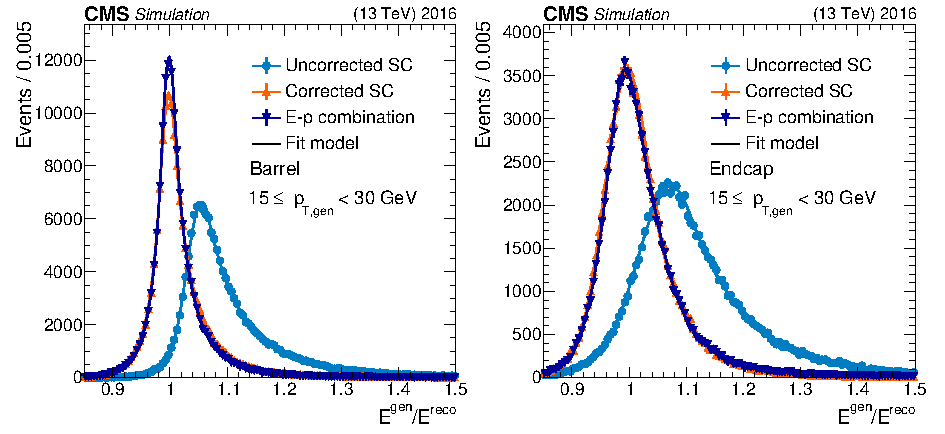
\includegraphics[width=\textwidth]{Figures/Detector/CMS/ecal_regression_performance.pdf}
  \caption[Electron Energy Corrections]{Ratio of the true to the reconstructed electron energy for $15 < \pt < 30$\GeV with and without regression corrections, and before and after the combination of the ECAL and tracker measurements, with a DCB function fit overlaid, in 2016 simulated events for barrel (left) and endcap (right) electrons. Vertical bars on the markers represent statistical uncertainties. Figure taken from Ref.~\cite{CMS:2020uim}.}\label{fig:ecal_regression_performance}
\end{figure}

After these simulation-based corrections, there are differences between data and simulation in the energy scales and resolutions of \eg objects. Further corrections are applied to correct the energy scale in data to match simulation, and since the resolution in simulation is better than that in data, smearings are applied to the simulation to match the data~\cite{CMS:2020uim}. These corrections are derived with $\PZ\rightarrow ee$ events by comparing the distribution of the invariant mass of the $\PZ$ boson in data and simulation. This is done in several stages. 

In the first stage, energy scale corrections are derived in about 18 hour intervals and in bins of $\eta$ corresponding to $0 < \abs{\eta} < 1$, $1.00 < \abs{\eta} < 1.44$, $1.57 < \abs{\eta} < 2.00$ and $2.00 < \abs{\eta} < 2.50$. The region, $1.44 < \abs{\eta} < 1.57$ represents the transition between the barrel and endcap regions and is not used. These initial corrections account for long-term drifts in the energy scale and accounts for $\eta$-dependent radiation damage. In the second stage, the energy scale and resolution is corrected in 50 categories, corresponding to 5 bins of $\eta$ and 10 bins of \RNINE. The magnitude of these corrections is up to 1.5\% and the systematic uncertainty associated with them is 0.05--0.1 (0.1--0.3)\% in the EB (EE), depending on the \RNINE bin~\cite{CMS:2020uim}. 

The final agreement between data and simulation in $Z\rightarrow ee$ events is shown in \cref{fig:zee_after_corrections} in two representative categories. The final energy resolution is found to be 2--5\%, depending on the $\eta$ and \RNINE of the electron~\cite{CMS:2020uim}. 

\begin{figure}
  \centering
  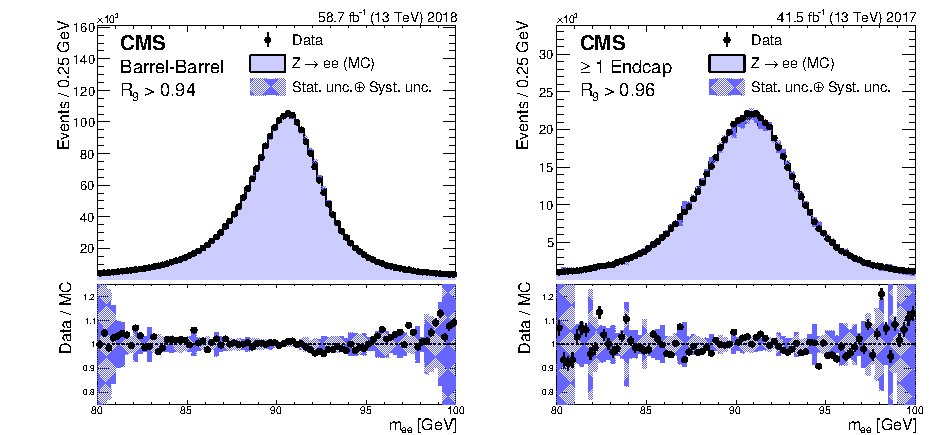
\includegraphics[width=\textwidth]{Figures/Detector/CMS/zee_after_corrections.pdf}
  \caption[Electron Energy Scale Agreement Between Simulation and Data]{Invariant mass distribution of the \PZ boson in $\PZ\to ee$ events, after scale and smearing corrections. Results are shown for barrel (left) and endcap (right) electrons in high \RNINE categories. The vertical bars on the markers represent the statistical uncertainties in data and the hatched regions show the combined statistical and systematic uncertainties in the simulation. The lower panels display the ratio of the data to the simulation with the bands representing the uncertainties in the simulation. Figure taken from Ref.~\cite{CMS:2020uim}.}\label{fig:zee_after_corrections}
\end{figure}
\subsection{Jets}\label{sec:jet_reco}
Quarks and gluons (partons) produced in a proton-proton collision shower and hadronize into collimated sprays of particles. To make a measurement of an outgoing parton, these particles are first clustered into \textit{jets} and the parton's properties are inferred from properties of the jet, such as its energy. In most CMS analyses, including the di-Higgs search in \cref{chap:dihiggs}, jets are reconstructed using the \akt algorithm~\cite{Cacciari:2008gp,Cacciari:2011ma} with a distance parameter of 0.4. 

Jet energy corrections are derived from simulation studies so that the energy of reconstructed jets match the energy of particle-level jets, where the difference between reconstructed jets and particle-levels jets is whether the jet constituents are reconstructed or taken directly from the generator (truth-level). Further corrections are made using dijet, \gjet, and $\PZ+\text{jet}$ events to account for differences between data and simulation~\cite{CMS:2016ljj,CMS-DP-2021-033}. The jet energy resolution for jets with $\pt=30$\GeV is about 15--25\% depending on the level of pileup, and improves to 10--15\% at $\pt=100$\GeV and 5\% at $\pt=1\TeV$~\cite{CMS-DP-2021-033}.

The identification of jets originating from \Pqb quarks (\Pqb jets) is performed used a deep neural network algorithm, DeepJet~\cite{CMS-DP-2018-058}. The algorithm uses properties of the particle-flow constituents of a jet as well information from associated secondary vertices. Three working points are defined: loose, medium, and tight, corresponding to a rate of misidentifying a light jet as a \Pqb jet of about 10\%, 1\% and 0.1\% respectively. 
\subsection{Tau Leptons}\label{sec:tau_reco}
\begin{table}
  \centering
  \begin{tabular}{llccc}
          \toprule
          & Decay mode & Resonance & \multicolumn{2}{c}{$\mathcal{B}$ (\%)} \\ 
          \midrule
          \multicolumn{2}{l}{Leptonic decays} & & 35.2 & \\
          & $\tau^- \to e^- \bar{\nu}_e \nu_\tau$ & & & 17.8 \\
          & $\tau^- \to \mu^- \bar{\nu}_\mu \nu_\tau$ & & & 17.4 \\
          \midrule
          \multicolumn{2}{l}{Hadronic decays} & & 64.8 & \\
          & $\tau^- \to h^- \nu_\tau$ & & & 11.5 \\
          & $\tau^- \to h^- \pi^0 \nu_\tau$ & $\rho(770)$ & & 25.9 \\
          & $\tau^- \to h^- \pi^0 \pi^0 \nu_\tau$ & $a_1(1260)$ & & 9.5 \\
          & $\tau^- \to h^-h^+h^ -\nu_\tau$ & $a_1(1260)$ & & 9.8 \\
          & $\tau^- \to h^-h^+h^- \pi^0 \nu_\tau$ & & & 4.8 \\
          & Other & & & 3.3 \\
          \bottomrule
  \end{tabular}
  \caption[Tau Lepton Decays and Branching Fractions]{Decays of $\tau$ leptons and their branching fractions ($\mathcal{B}$). Where appropriate, the known intermediate resonances for a decay are indicated. Charged hadrons are denoted by the symbol $h^\pm$ and although only $\tau^-$ decays are shown, the values are also valid for the charge-conjugated processes.}\label{tab:tau_decays}
\end{table}

Tau leptons decay into a variety of final states, which are summarized in \cref{tab:tau_decays}. About one third of the time, tau leptons decay \textit{leptonically} into an electron or muon, and two neutrinos. In such a decay, the electrons and muons are reconstructed as described in \cref{sec:eg_reco,sec:muon_reco}, and properties of the neutrinos are inferred from the missing transverse momentum. The other two thirds of the time, tau leptons decay \textit{hadronically} into hadrons and a neutrino. These types of tau leptons, denoted \tauh, are reconstructed with the hadrons-plus-strips (HPS) algorithm. 

\subsubsection{Hadrons-Plus-Strips Algorithm}

The HPS algorithm~\cite{CMS:2015pac,CMS:2018jrd} begins by searching the constituents of reconstructed jets for charged hadrons and neutral mesons. A $\pi^0$ meson promptly decays into two photons, which are then likely to convert into $e^+e^-$ pairs as they traverse the tracker material. The energy of the $\pi^0$ meson is therefore spread over a $\Delta\eta \times \Delta\phi$ region which is referred to as a \textit{strip}. The basic ingredients of the HPS algorithm are charged hadrons and strips, hence the name.

A strip is reconstructed by clustering electrons and photons inside a jet, and begins by seeding the strip with the highest \pt electron or photon in the jet. Then, a $\Delta\eta \times \Delta\phi$ area centred on the seed is defined and the next-highest \pt electron or photon inside the area is added to the strip. The strip position, which was originally defined by the seed, is then recomputed using a \pt-weighted average of all electrons and photons in the strip and the process is repeated until no more electrons or photons can be added.

The size of the $\Delta\eta \times \Delta\phi$ area is dynamic and is dependent on the \pt of the strip and of the candidate electron or photon to account for several effects~\cite{CMS:2018jrd}. Firstly, the likelihood of a photon converting into an $e^+e^-$ pair is higher at lower \pt, so the strip size is expected to be larger for lower \pt strips. Furthermore, the decay products for a \tauh with higher \pt tend to be boosted in the direction of the \tauh, leading to a smaller strip. The functions used to define the strip size are derived from simulation of \tauh decays and are designed such that 95\% of all electrons and photons arising from a \tauh decay are included in the strip.

Based on the set of charged hadrons and strips in a jet, the HPS algorithm identifies the decay mode from \cref{tab:tau_decays}. To reduce misidentification with jets, the mass of the sum of the hadron candidates is required to be compatible with a $\rho(770)$ or $a_1(1260)$ resonance, depending on the decay mode. Additionally, $\tau_h$ candidates are required to have a charge of $\pm1$, and to have no charged particles or strips outside a signal cone, defined by $R_{\text{sig}} = (3.0\GeV)/\pt$, where the \pt is that of the hadronic system, and the cone size is limited to 0.05--0.10. Finally, a single $\tau_h$ candidate is allowed per jet by selecting the candidate with the highest \pt. The \tauh reconstruction efficiency is measured in data with $\PZ\to\tau\tau$ events and is found to be about 75\% for \tauh with $\pt > 30$\GeV~\cite{CMS:2022prd}. 

\subsubsection{DeepTau ID}\label{sec:tau_deeptau_id}

The DeepTau ID algorithm~\cite{CMS:2022prd} is a deep neural network that is used to identify \tauh candidates and reject jets, electrons and muons misidentified as \tauh candidates. The algorithm uses a combination of higher-level inputs, which are summary variables related to the \tauh candidate, and lower-level inputs, which are variables related to reconstructed particles in the vicinity of the \tauh candidate. Higher-level inputs include the \tauh four momentum, number of charged and neutral particles used to reconstruct the \tauh candidate, and isolation variables. To construct the lower-level inputs, particles within a $\Delta\eta \times \Delta\phi = 0.05 \times 0.05$ area centred around the \tauh candidate are considered, and properties such as the particle type, \pt, $\eta$, $\phi$, charge, and compatibilities with primary and secondary vertices are included.

The network is a multiclassifier with four outputs: jet, $\mu$, $e$, and \tauh, and it is trained with a modified cross-entropy loss function on simulated events from the following processes: $\PZ+\text{jets}$, $\PW+\text{jets}$, $t\bar{t}$, QCD multijet production, and $\PZ^'\to\tau\tau$, $\PZ^'\to ee$ and $\PZ^'\to \mu\mu$ where $1 < m_{\PZ^'} < 5$\TeV. The final discriminators against jets, muons, and electrons are given by:
\begin{equation}
  \Dalpha = \frac{y_\tau}{y_\tau + y_\alpha}
\end{equation}
where $\alpha \in \{\text{jet}, \mu, e\}$ and $y_i$ are the four outputs of the network. Working points are defined for each discriminator based upon the expected \tauh identification efficiencies as measured in $\PH\to\tau\tau$ events for \tauh candidates with $30 < \pt < 70$\GeV. These working points are summarized in \cref{tab:deeptau_working_points}.

\begin{table}
	\centering
	\begin{tabular}{lcccccccc}
		& VVTight & VTight & Tight & Medium & Loose & VLoose & VVLoose & VVVLoose \\ \midrule
		\De & 60\% & 70\% & 80\% & 90\% & 95\% & 98\% & 99\% & 99.5\% \\
		\Dm & --- & --- & 99.5\% & 99.8\% & 99.9\% & 99.95\% & --- & --- \\
		\Djet & 40\% & 50\% & 60\% & 70\% & 80\% & 90\% & 95\% & 98\% \\
	\end{tabular}
  \caption[Identification Efficiencies at Different DeepTau ID Working Points]{Target \tauh identification efficiencies for different working points defined for the three different discriminators. The target efficiencies are evaluated with simulated $\PH\to\tau\tau$ events for \tauh with $\pt \in [30, 70]\GeV$.}\label{tab:deeptau_working_points}
\end{table}

The combined efficiency of \tauh reconstruction and identification as measured in different bins of \tauh \pt with simulated $\PZ\to\tau\tau$ decays is shown in \cref{fig:tau_reco_id_eff}. After applying the Loose, Medium or Tight \Djet working points, the efficiency increases with \tauh \pt and for $\pt > 30$\GeV, the efficiency is above 40\%, 50\%, and 60\% for the respective working points. The corresponding misidentification rates for jets, electrons, and muons as a function of the \tauh identification efficiency are shown in \cref{tab:deeptau_misid_rates}. At a \tauh identification efficiency of 80\%, the misidentification rate for electrons is about 0.1\%, for muons is less than 0.03\%, and for jets is between 1 and 4\%, depending on \tauh \pt.

\begin{figure}
  \centering
  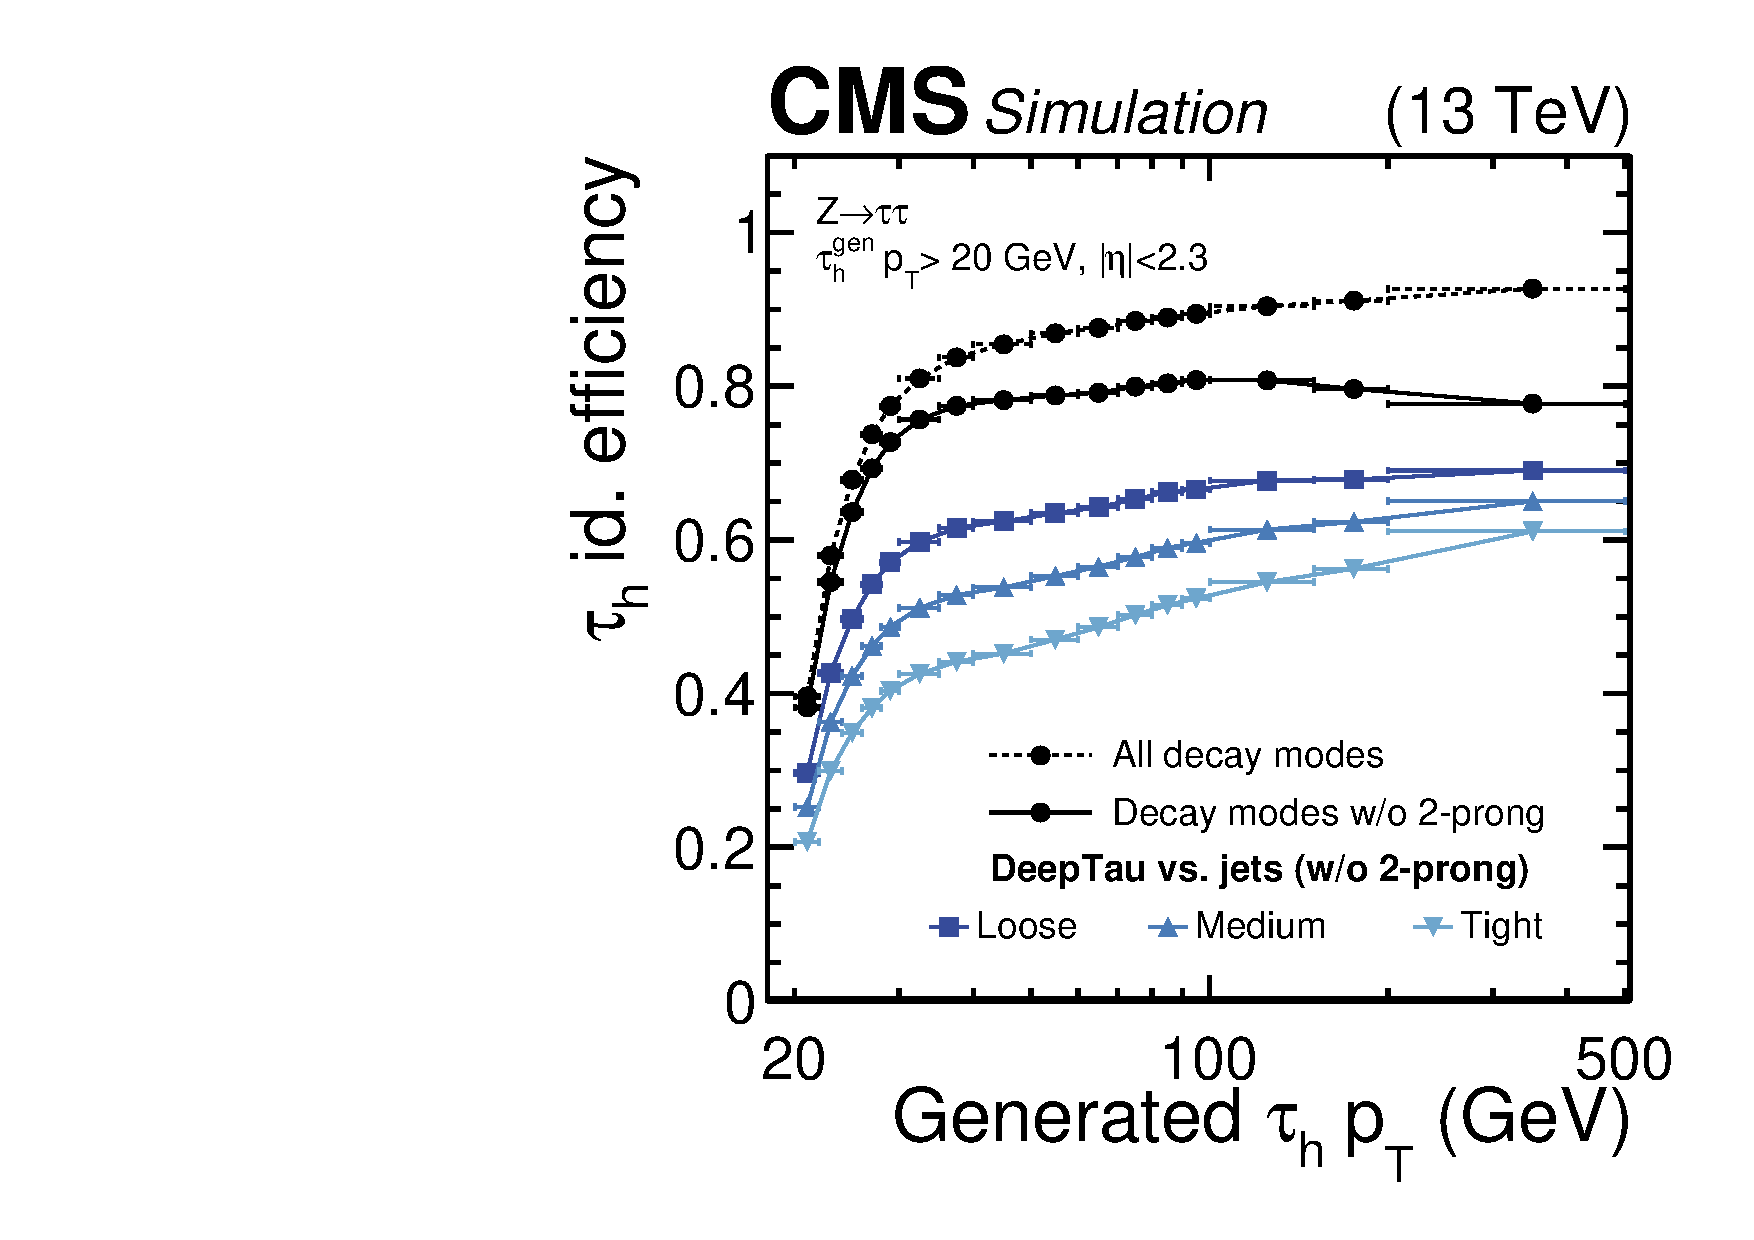
\includegraphics[width=0.49\textwidth]{Figures/Detector/CMS/tau_reco_id_eff.pdf}
  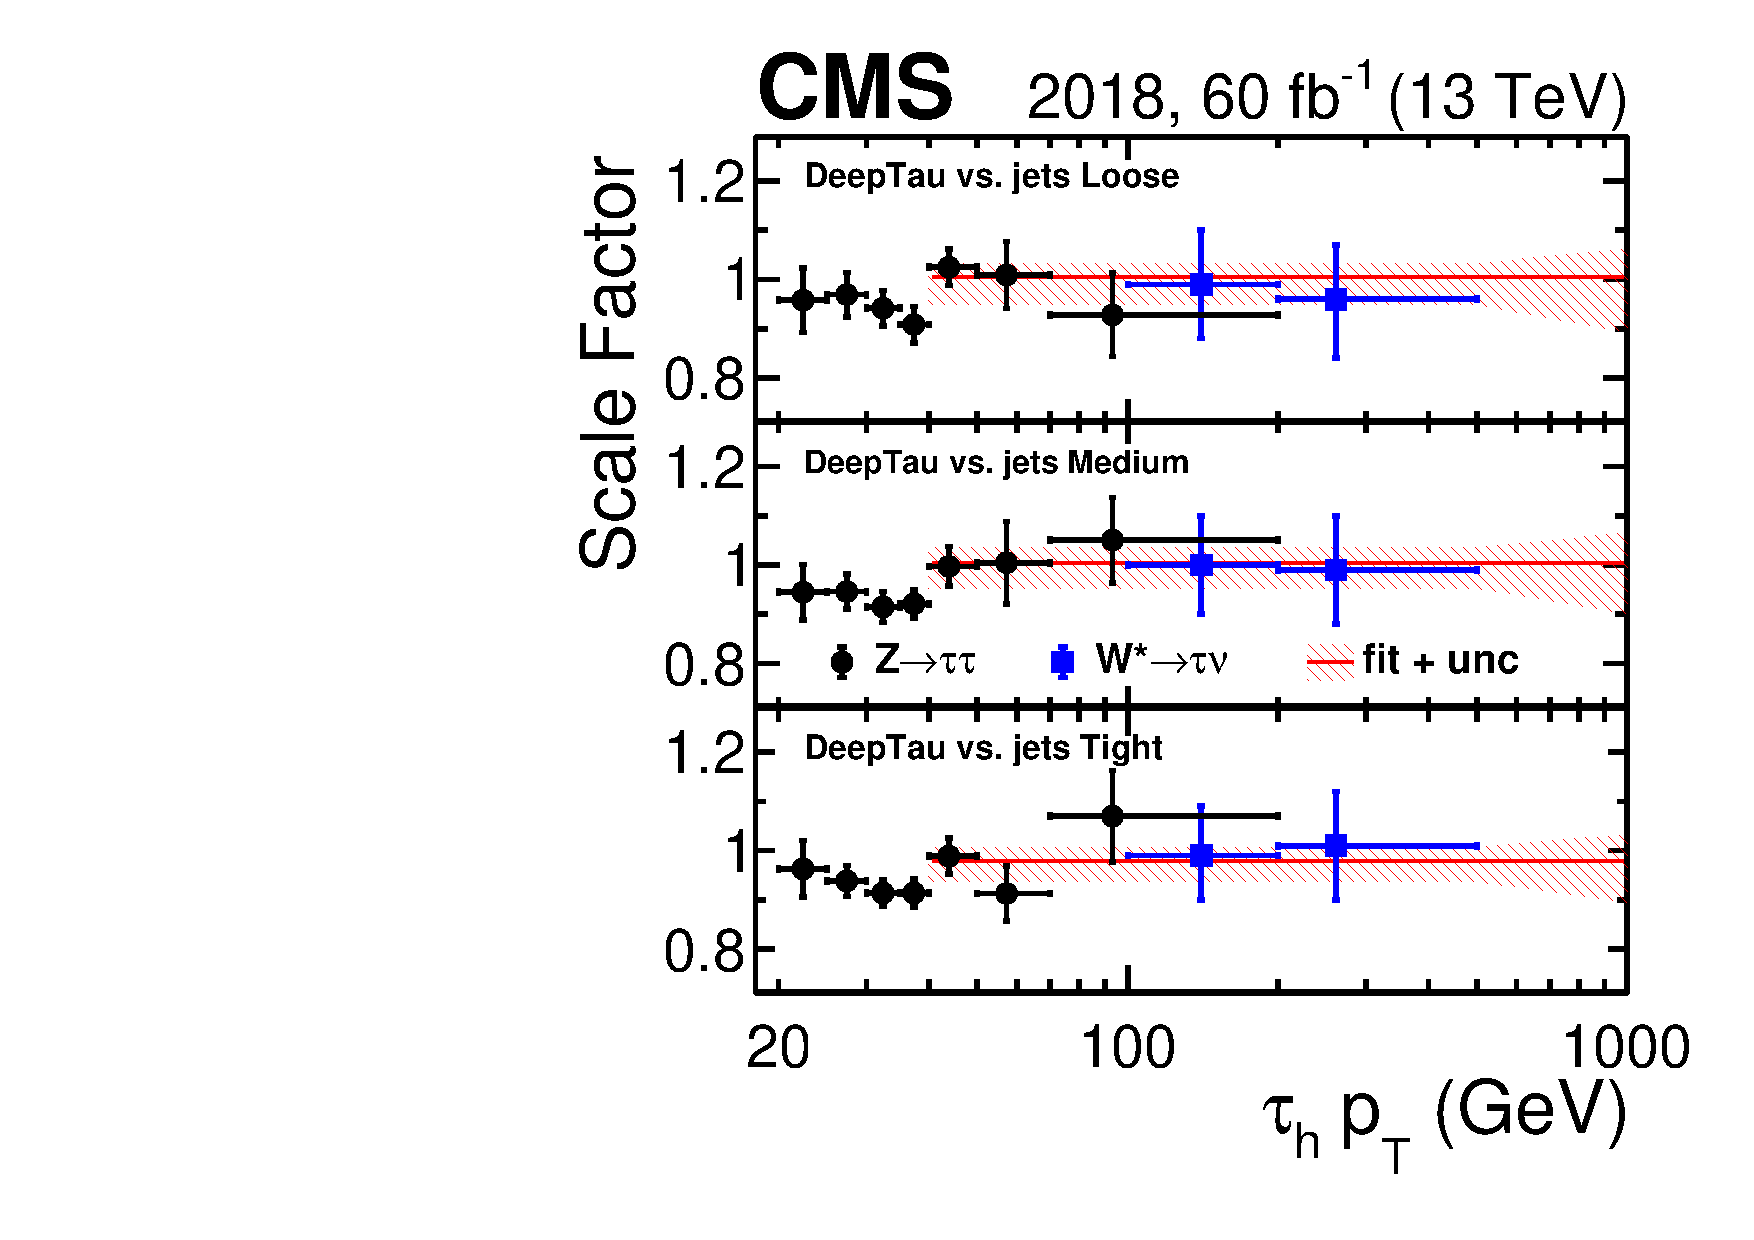
\includegraphics[width=0.49\textwidth]{Figures/Detector/CMS/tau_id_scale_factor.pdf}
  \caption[\tauh Reconstruction and Identification Efficiency]{Reconstruction and identification efficiency of \tauh candidates as measured in simulated $Z\to\tau\tau$ events (left) and corresponding scale factors measured with data collected in 2018 (right). In both plots, the results are shown as functions of the true (generated) \tauh \pt, and the efficiencies after applying the Loose, Medium and Tight DeepTau ID working points are calculated after excluding 2-prong decays, which are those containing missing charged hadrons. In the right plot, the vertical bars represent combined statistical and systematic uncertainties in the scale factors, and the red line and hatched region represents a constant fit to the scale factors for $\pt > 40$\GeV and the associated uncertainty. Figures taken from Ref.~\cite{CMS:2022prd}.}\label{fig:tau_reco_id_eff}
\end{figure}

\begin{figure}
  \centering
  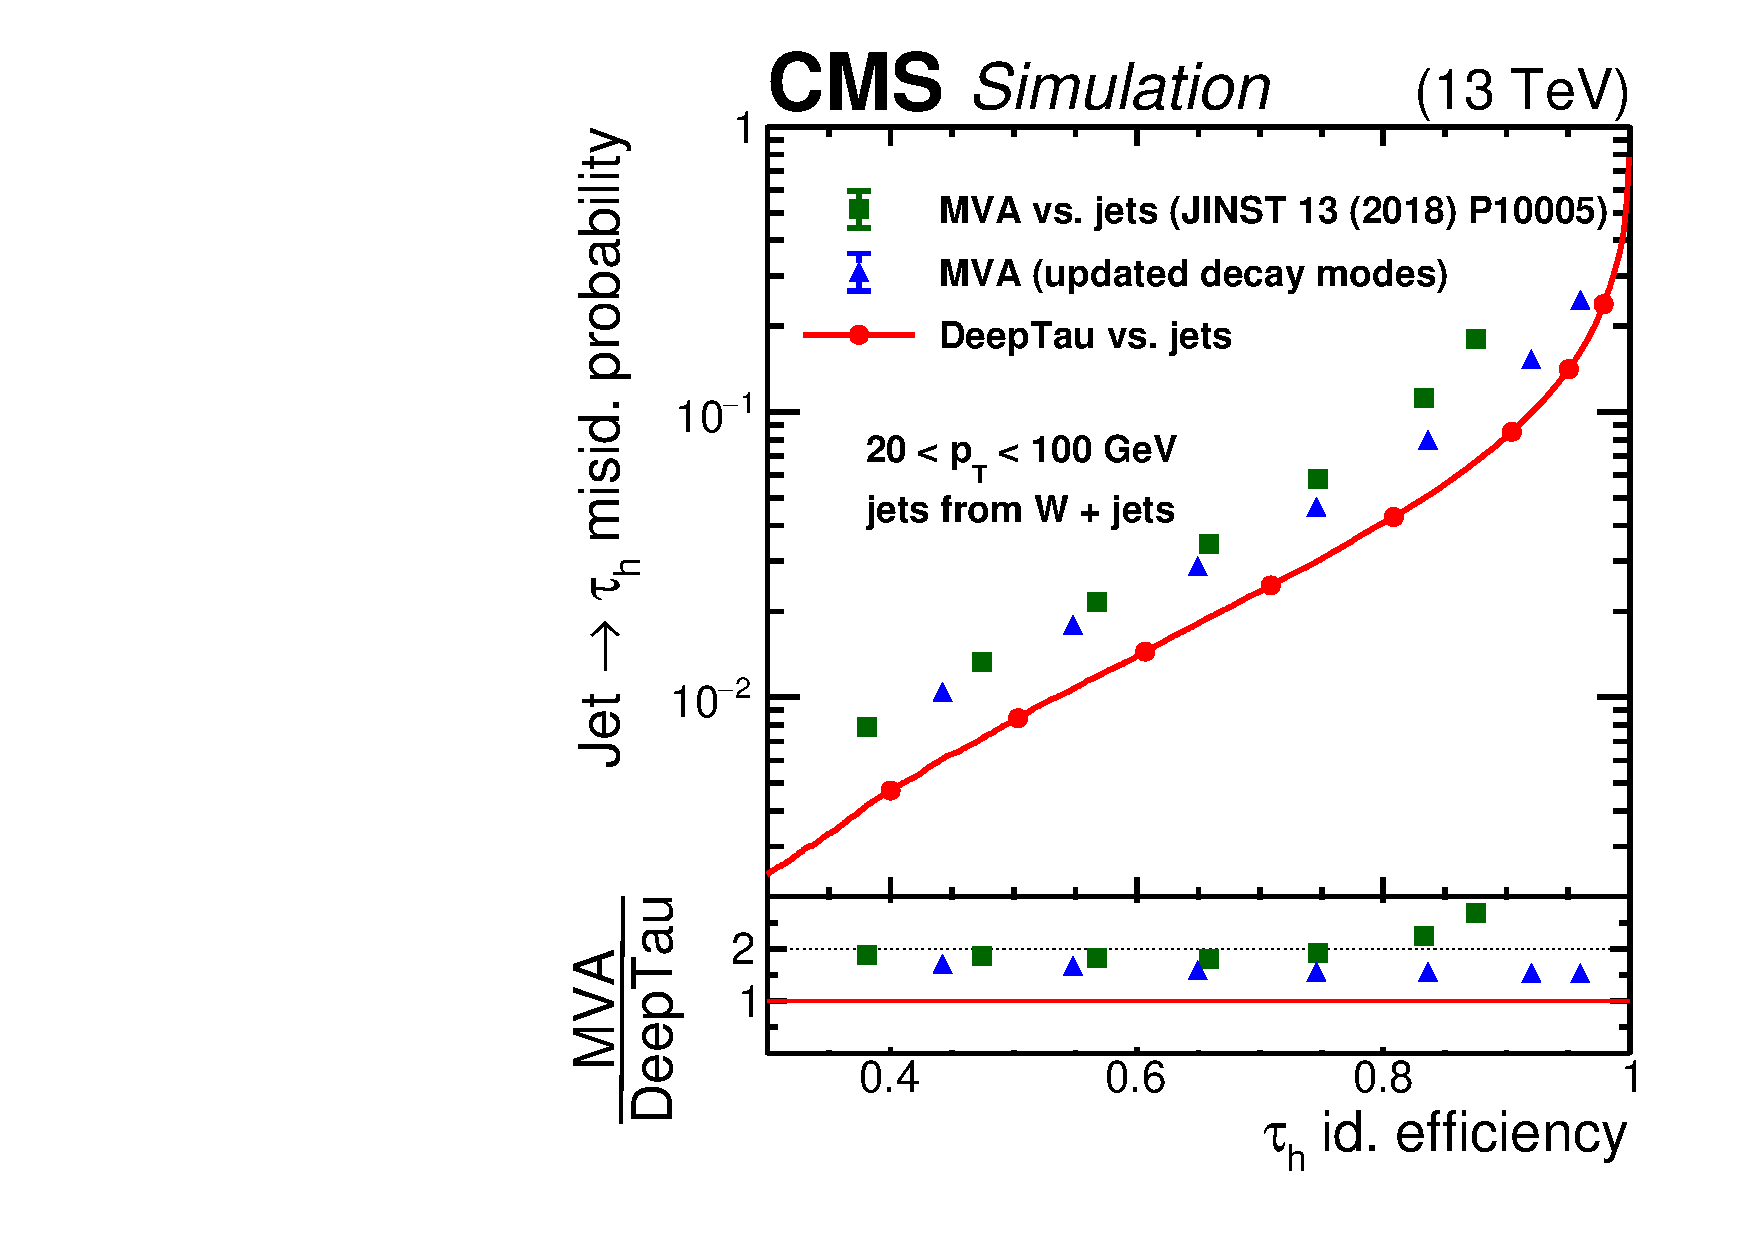
\includegraphics[width=0.49\textwidth]{Figures/Detector/CMS/tau_id_jet_misid_wjet_20_100.pdf}
  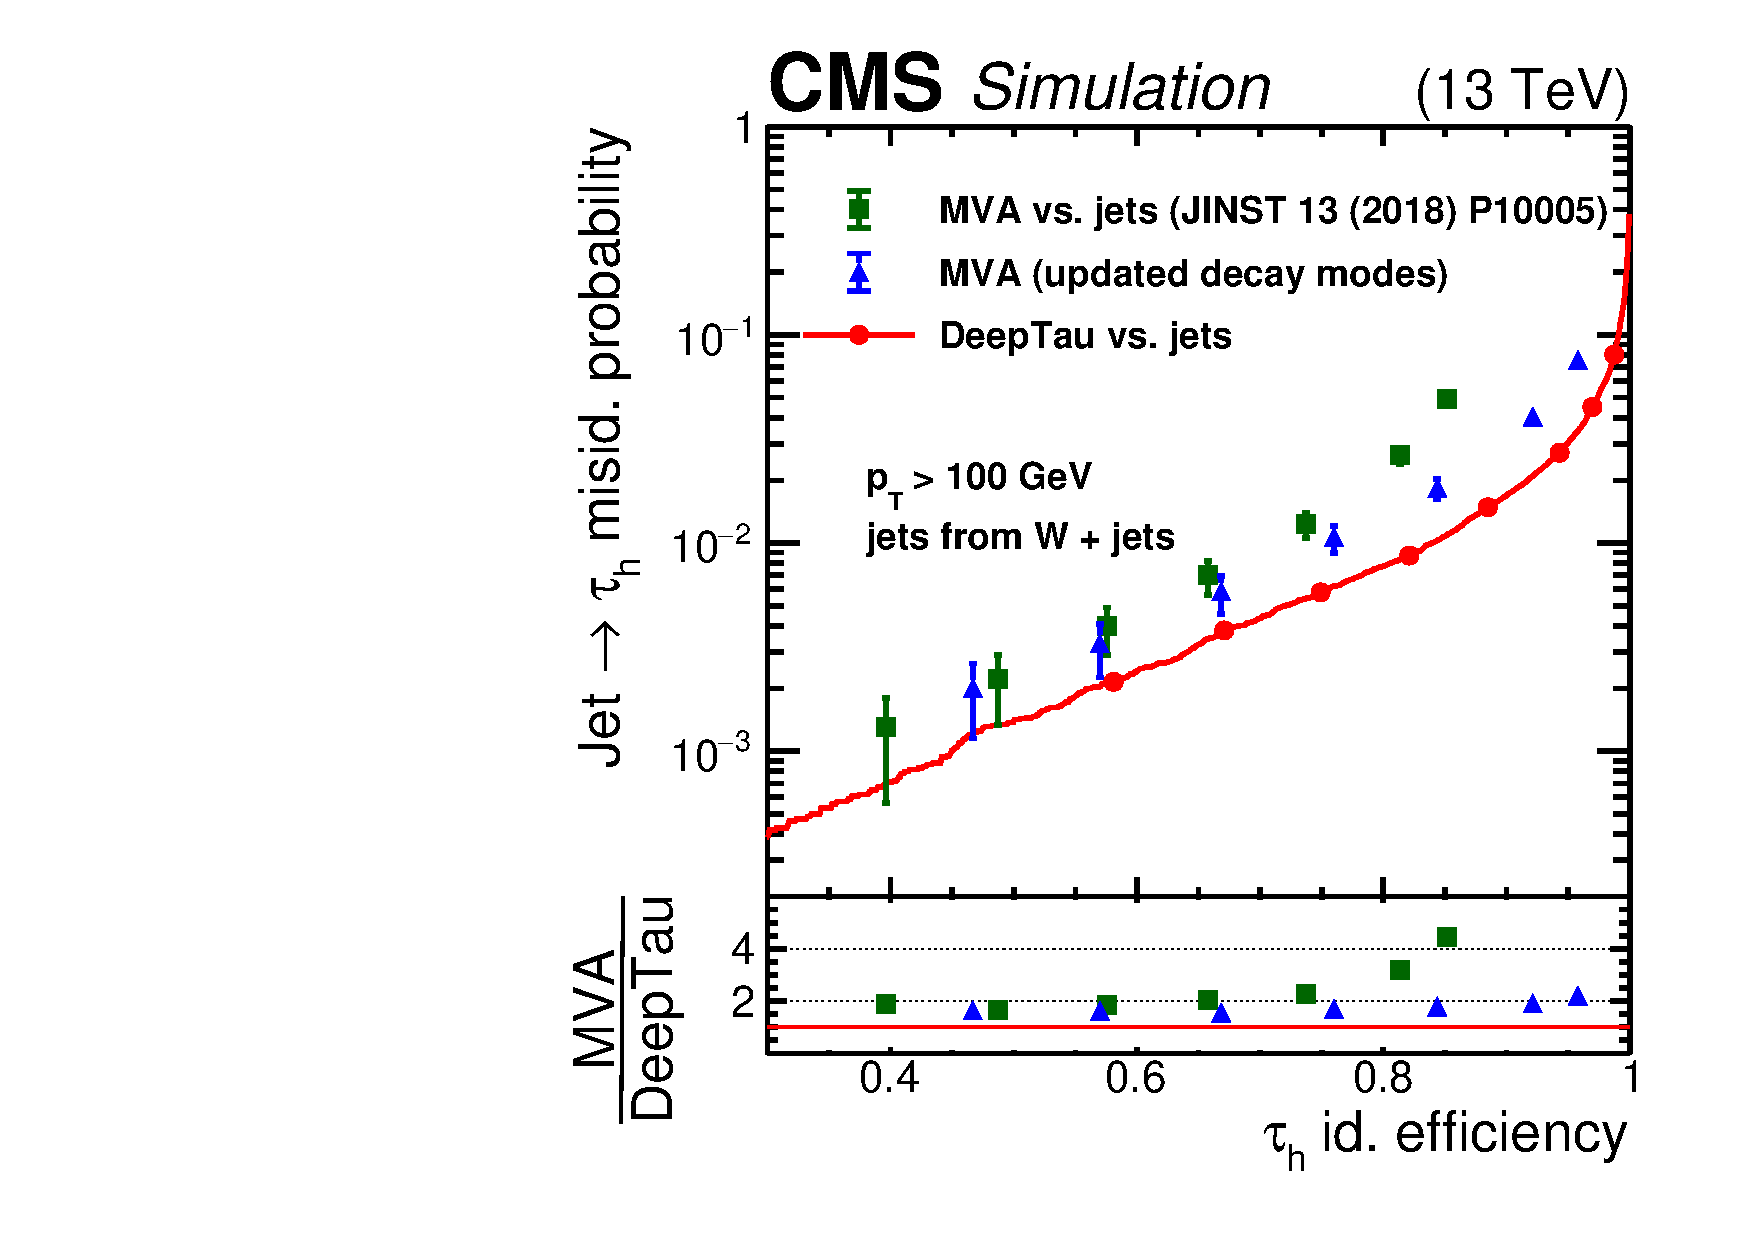
\includegraphics[width=0.49\textwidth]{Figures/Detector/CMS/tau_id_jet_misid_wjet_gt100.pdf}
  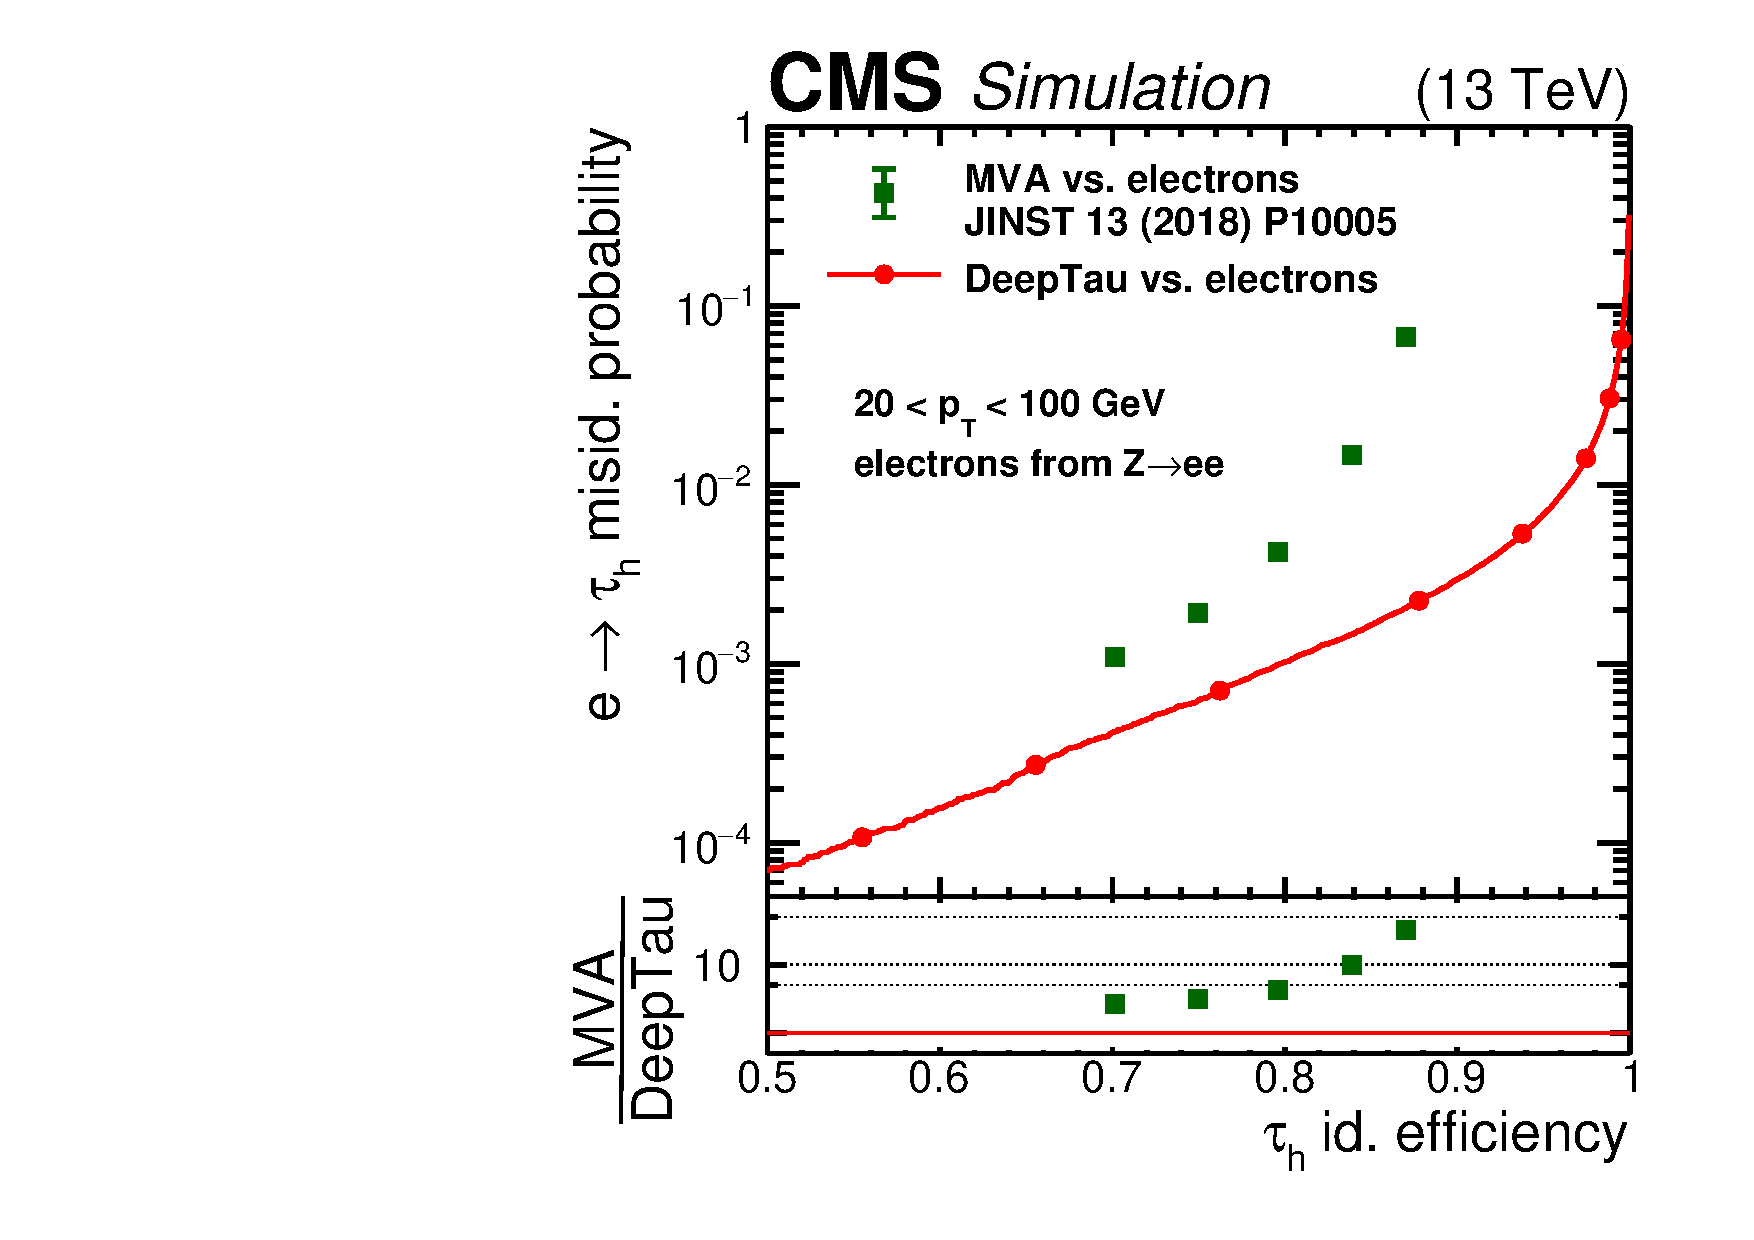
\includegraphics[width=0.49\textwidth]{Figures/Detector/CMS/tau_id_e_misid_20_100.pdf}
  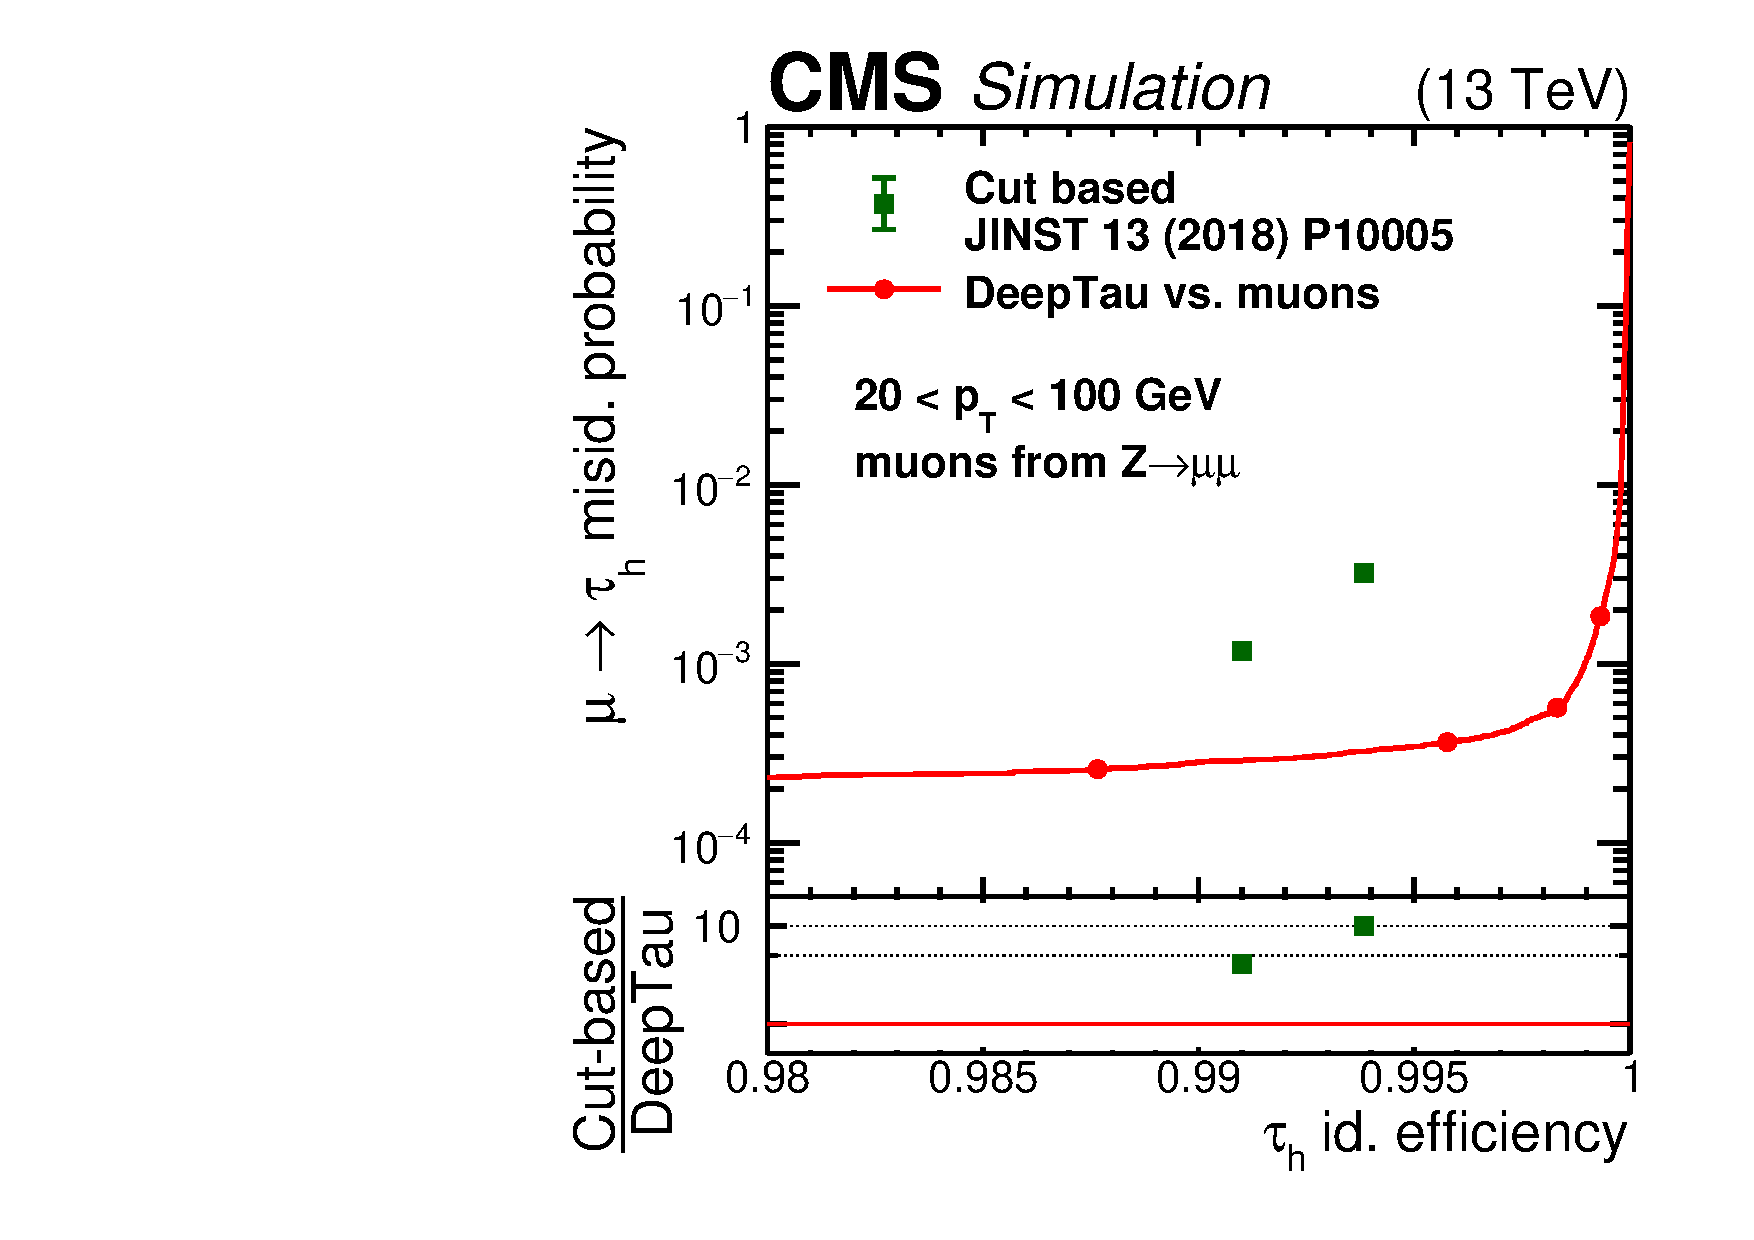
\includegraphics[width=0.49\textwidth]{Figures/Detector/CMS/tau_id_mu_misid_20_100.pdf}
  \caption[Performance of the DeepTau ID Algorithm]{Misidentification rates for jets (top), electrons (bottom left), and muons (bottom right) as a function of the \tauh identification efficiency for the \Djet, \De, and \Dm discriminators respectively. Also shown is the performance of previous \tauh identification algorithms and the ratio of misidentification rates between one of the alternate algorithms and DeepTau is shown in the bottom half of each plot. In all cases, DeepTau outperforms the alternate algorithm. For jets, efficiencies are shown for jets with $20 < \pt < 100$\GeV (top left) and $\pt>100$\GeV (top right) and they indicate that higher \pt jets are less likely to be misidentified. For electrons and muons, the efficiencies are only shown for $20 < \pt < 100$\GeV since the misidentification rate is approximately constant with \pt for these objects. Vertical bars represent statistical uncertainties and the full red circles represent the working points. Figures taken from Ref.~\cite{CMS:2022prd}.}\label{tab:deeptau_misid_rates}
\end{figure}

The \tauh reconstruction and identification efficiencies are also measured in data with $Z\to\mu\tauh$ and $W^*\to\nu\tauh$ events~\cite{CMS:2022prd} and scale factors are derived to correct the simulation to match data. These scale factors are derived in bins of \pt and their values and uncertainties are shown in \cref{fig:tau_reco_id_eff}. The corrections are at most 10\% and have an uncertainty of 2--5\%~\cite{CMS:2022prd}.

\subsubsection{\tauh Energy Scale}\label{sec:tau_energy_scale}

The \tauh energy scale is measured in data with $\mu\tauh$ events by fitting the distributions of the $\mu\tauh$ invariant mass, \mvis, and the reconstructed \tauh mass, \mtauh. Simulated templates of the \mvis and \mtauh distributions are created for \tauh energy shifts between $\pm3\%$ in steps of 0.2\% and a maximum likelihood fit is performed for each shift. This is performed in bins of the \tauh decay mode and separately for \mvis and \mtauh. The corresponding energy scale corrections are shown in \cref{fig:tau_energy_scale} and are found to be up to 2\% with uncertainties of 0.6--0.8\% depending on decay mode. The results from measuring \mvis and \mtauh are found to be consistent with each other and the final energy scale corrections are derived from a combination of the two approaches. After applying the corrections, good agreement is found in the \mvis and \mtauh distributions as shown in \cref{fig:tau_energy_scale_fit}.

\begin{figure}
  \centering
  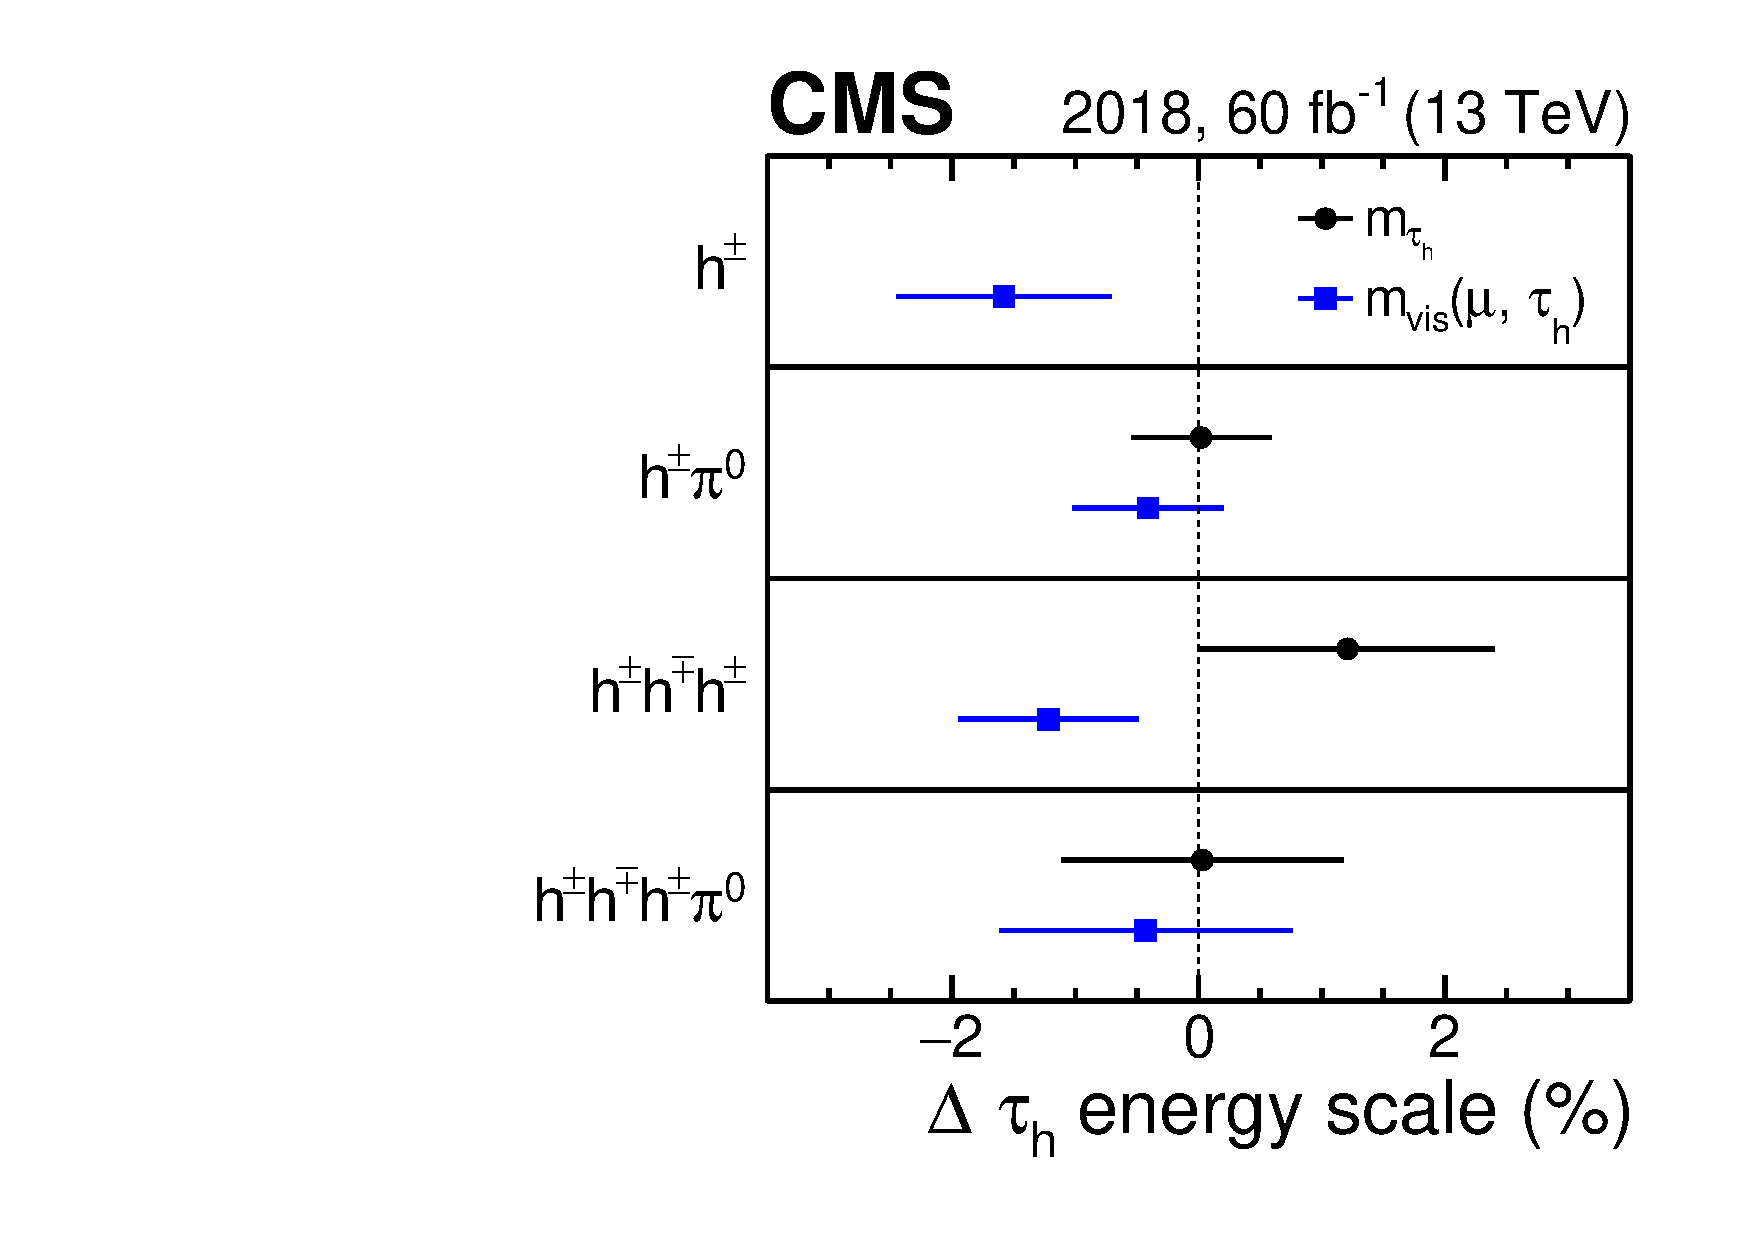
\includegraphics[width=0.5\textwidth]{Figures/Detector/CMS/tau_energy_scale.pdf}
  \caption[\tauh Energy Scale Corrections]{Relative difference for the \tauh energy obtained between data and simulated events for 2018 for the four main reconstructed \tauh decay modes. The results are obtained from fits to the distribution of either the reconstructed \mvis (blue lines) or \mtauh (black lines). The horizontal bars represent the combined statistical and systematic uncertainties in the measurements. Figure taken from Ref.~\cite{CMS:2022prd}.}\label{fig:tau_energy_scale}
\end{figure}

\begin{figure}
  \centering
  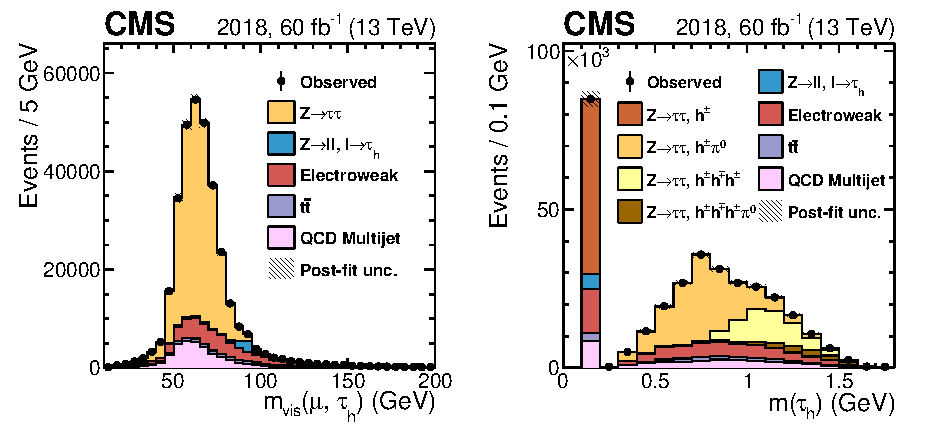
\includegraphics[width=\textwidth]{Figures/Detector/CMS/tau_energy_scale_fits.pdf}
  \caption[\tauh Energy Scale Agreement Between Simulation and Data]{Distribution of the reconstructed visible invariant mass of the $\mu\tauh$ system, \mvis (left) and of the visible invariant \tauh mass (right) in 2018 data (black dots) and simulated events (filled histograms). Vertical bars correspond to statistical uncertainties. The \tauh is required to pass the Tight \Djet working point, and have $\pt > 20$\GeV and $\abs{\eta}<2.3$. The distributions incorporate all measured scale factors and energy corrections and are scaled to the outcome of a maximum likelihood to the observed data with the $\PZ\to\tau\tau$ contribution freely floating. In the $m(\tauh)$ distribution, the $\PZ\to\tau\tau$ contributions are shown separately for the different \tauh decay modes. Figures taken from Ref.~\cite{CMS:2022prd}.}\label{fig:tau_energy_scale_fit}
\end{figure}


\subsection{Summary}
Object reconstruction at the CMS experiment is a complex process that involves dedicated algorithms for each type of object, often combining information from different subdetectors to maximize performance. All the reconstruction algorithms described in this Section have some relevance to the di-Higgs search presented in \cref{chap:dihiggs} but the most relevant are those for the photons and \tauh objects. The excellent ECAL energy resolution leads to a resolution of about 1\% on the diphoton invariant mass, \mgg, for values of \mgg around 125\GeV. In \Hgg analyses, this leads to a narrow signal peak in the \mgg distribution which is used to identify the signal above a large background. On the \tauh side, signal is separated from background using the Loose \Djet WP which identifies \tauh candidates with an 80\% efficiency whilst maintaining a jet misidentification rate between 1\% and 4\% depending on the \tauh \pt.